        %%******************************************%%
        %%                                          %%
        %%        Modello di tesi di laurea         %%
        %%            di Andrea Giraldin            %%
        %%                                          %%
        %%             2 novembre 2012              %%
        %%                                          %%
        %%******************************************%%

\begin{document}
    \frontmatter
    \begin{titlepage}
    \begin{center}
        \begin{LARGE}
            \textbf{\myUni}\\
        \end{LARGE}

        \vspace{10pt}

        \begin{Large}
            \textsc{\myDepartment}\\
        \end{Large}

        \vspace{10pt}

        \begin{large}
            \textsc{\myFaculty}\\
        \end{large}

        \vspace{30pt}
        \begin{figure}[htbp]
            \centering
            
\includegraphics[height=6cm]{unipd-logo}
        \end{figure}
        \vspace{30pt}

        \begin{LARGE}
            \textbf{\myTitle}\\
        \end{LARGE}

        \vspace{10pt}

        \begin{large}
            \textsl{\myDegree}\\
        \end{large}

        \vspace{40pt}

        \begin{large}
            \begin{flushleft}
                \textit{Relatrice}\\
                \vspace{5pt}
                \profTitle\ \myProf
            \end{flushleft}

            % You can tweak the spacing to have professor and student names on the same line
            % useful if the page is broken by a long thesis title and you need more space
            % \vspace{-52pt}

            \begin{flushright}
                \textit{Laureando}\\
                \vspace{5pt}
                \myName \\
                \vspace{5pt}
                Matricola: \myMatricola
            \end{flushright}
        \end{large}

        \vspace{28pt}

        \line(1, 0){338} \\
        \begin{normalsize}
            \textsc{Anno Accademico \myAA}
        \end{normalsize}
    \end{center}
\end{titlepage}

    \clearpage
\phantomsection
\thispagestyle{empty}

\hfill
\vfill

\noindent\myName: \textit{\myTitle,}
\myDegree,
\textcopyright\ \myTime.

    \cleardoublepage
\phantomsection
\thispagestyle{empty}
\pdfbookmark{Dedica}{Dedica}

\vspace*{3cm}

\begin{center}
    Leave a Little Sparkle wherever you go. \\ \medskip
\end{center}

\medskip

\begin{center}
    Dedicato a tutti coloro che ci sono stati vicini nei momenti più difficili.
\end{center}

    \cleardoublepage
\phantomsection
\pdfbookmark{Sommario}{Sommario}
\begingroup
\let\clearpage\relax
\let\cleardoublepage\relax
\let\cleardoublepage\relax

\chapter*{Sommario}

Il presente documento descrive il lavoro svolto durante il periodo di stage, della durata di circa trecento ore, dal laureando Marco Brugin presso l'azienda Sybclab S.r.L.
Gli obbiettivi da raggiungere sono stati:
in primo luogo è stata richiesta la comprensione dei vantaggi e degli overhead portati da una architettura Event Driven,
in secondo luogo è stata richiesta la comprensione e implementazione di una data pipeline con il trattamento dei dati tramite Apache Kafka e Apache Druid ed infine la comprensione e la gestione gestione delle Time Series e dei Column-based Databases.
Il prototipo sviluppato presenterà una architettura distribuita, ad alta affidabilità, scalabile e resiliente, eseguibile tramite Docker Compose.
%\vfill

%\selectlanguage{english}
%\pdfbookmark{Abstract}{Abstract}
%\chapter*{Abstract}

%\selectlanguage{italian}

\endgroup

\vfill

    \cleardoublepage
\phantomsection
\pdfbookmark{Ringraziamenti}{ringraziamenti}

\begin{flushright}{
    \slshape
    ``Life is really simple, but we insist on making it complicated''} \\
    \medskip
    --- Confucius
\end{flushright}


\bigskip

\begingroup
\let\clearpage\relax
\let\cleardoublepage\relax
\let\cleardoublepage\relax

\chapter*{Ringraziamenti}

\noindent \textit{Innanzitutto, vorrei esprimere la mia gratitudine al Prof. \myProf, relatore della mia tesi, per l'aiuto e il sostegno fornitomi durante la stesura del lavoro.}\\

\noindent \textit{Desidero ringraziare con affetto i miei genitori per il sostegno, il grande aiuto e per essermi stati vicini in ogni momento durante gli anni di studio.}\\

\noindent \textit{Ho desiderio di ringraziare poi i miei amici per tutti i bellissimi anni passati insieme e le mille avventure vissute.}\\
\bigskip

\noindent\textit{\myLocation, \myTime}
\hfill \myName

\endgroup

    \cleardoublepage
\pdfbookmark{\contentsname}{tableofcontents}
\setcounter{tocdepth}{2}
\tableofcontents
%\markboth{\contentsname}{\contentsname}
\clearpage

\begingroup
    \let\clearpage\relax
    \let\cleardoublepage\relax
    \let\cleardoublepage\relax

    % Figures list
    \phantomsection
    \pdfbookmark{\listfigurename}{lof}
    \listoffigures

    \vspace*{8ex}

    % Tables list
    \phantomsection
    \pdfbookmark{\listtablename}{lot}
    \listoftables

    \vspace*{8ex}
\endgroup

\cleardoublepage

    \cleardoublepage

    \mainmatter
    \chapter{Introduzione}
\label{cap:introduzione}
\section{Descrizione dell'azienda}
Sync Lab s.r.L. è una azienda italiana attiva nell'abito \gls{ict}{}, specializzata nello sviluppo e consulenza IT dal 2002 con sedi a 
Milano, Roma, Napoli, Verona e Como. È una azienda orientata verso la Business Innovation, finalizzata alla 
creazione di soluzioni innovative che abbracciano i nuovi paradigmi della trasformazione digitale.
Sync Lab possiede numerose certificazioni ISO LL-C per l'attestazione della 
qualità dei prodotti e servizi offerti. In particolare possiede le certificazioni 
ISO-9001 per la qualità dell'azienda, ISO-14001 per l'adozione quadro sistematico per l'integrazione delle pratiche a protezione dell'ambiente, ISO-27001 per la definizione di un \gls{sgsi}{}, ISO-45001 per l'adozione di un \gls{ohs}{}.
\\
Attualmente Sync Lab dal punto di vista dell'organico è composta da più 300 dipendenti e lavora per più di 150 clienti diretti e finali, tra i più rilevanti ci sono nomi come: TIM, Trenitalia, PosteItaliane, UniCredit, ENI, ENEL, Vodafone, Fastweb.
\\
Sync Lab è un'azienda che si pone come obiettivo quello di essere un punto di riferimento per i propri clienti nella realizzazione di prodotti e soluzioni innovative per diversi settori di mercato, come mostrato  tra i quali: Sanità, Industria, Energia, Telco, Finanza e Trasporti \& Logistica.\\
Lo spirito di Sync Lab è ampiamente rappresentato dal logo aziendale Figura \ref{figure:logo_azienda}, che rappresenta un'onda che si propaga in modo circolare, che simboleggia la capacità di adattarsi e di evolversi in modo continuo.\\


\begin{figure}[htbp]  
\centering
    
\includegraphics[width=0.5\textwidth]{images/introduzione/logo_azienda.png}
    \caption{Logo dell'aziedan Sync Lab s.r.L.}
    \label{figure:logo_azienda}
\end{figure}
\pagebreak
\section{Idea di fondo del progetto}
Oggigiorno la gestione e l'analisi di grandi moli di dati in tempo reale sta diventando fondamentale 
per le aziende che vogliono rimanere competitive sul mercato. \\ 
Per questo motivo è necessario utilizzare tecnologie e software che permettano di analizzare e archiviare 
i dati in modo efficiente e veloce. \\
D'altro canto, però, è necessario anche che queste tecnologie siano in grado di scalare in modo verticale e orizzontale in base al carico 
di lavoro da sostenere. Inoltre è necessario che queste tecnologie siano in grado di garantire un elevato livello affidabilità. \\
Per questo motivo Sync Lab ha deciso d' investire in un progetto di ricerca e sviluppo che ha come obiettivo quello di creare 
una \gls{Data Pipeline}{} in grado di garantire le caratteristiche sopra descritte. \\
L'azienda ha già a disposizione un sistema di raccolta dati in  real time, basato su Apache Kafka, che permette di ricevere dati da
diversi sistemi e applicazioni, ma vuole andarlo a integrare con un sistema di analisi in real time permetta di eseguire operazioni 
sui dati ricevuti prima di archiviarli. \\
Particolarmente importante dovrà essere la fase di analisi dei dati, in quanto dovrà essere possibile eseguire operazioni di aggregazione
per aumentare la successiva estrazione dei dati. 
\subsection{Il ruolo dello stagista}
Lo stagista ha un ruolo fondamentale in tale tipologia di progetto, infatti è colui che porta uno spirito d'innovazione e consolida il valore aggiunto 
aziendale. \\
Le attività che costituiscono il percorso che lo stagista ha intrapreso sono state elencate all'interno di un \textit{Piano di lavoro}, che ha aiutato il tutor 
aziendale designato da Sync Lab a guidare e valutare il lavoro svolto dallo stagista. \\
Inoltre al termine del periodo di stage, sotto la supervisione del tutor aziendale è stata pianificata una presentazione rivolta a tutti \textit{stakeholder} aziendali, mirata a 
mostrare i risultati ottenuti con le tecnologie utilizzate e mettere in risalto le potenzialità del prototipo sviluppato. D'altra parte tale presentazione è stata anche l'occasione 
per un confronto per far emergere eventuali criticità o difetti,  e miglioramenti da apportare al prototipo sviluppato.
\pagebreak
\section{Il progetto di stage}
\subsection{Descrizione del progetto}
Le attività descritte in questa tesi si basano sulla progettazione e realizzazione di un prototipo di \gls{Data Pipeline}{} in grado di ricevere dati in real time da un sistema di raccolta dati basato su Apache Kafka, eseguire operazioni di aggregazione con Apache Druid in modo efficiente per facilitarne la successiva estrazione, fornendo così in output dati pronti per l'analisi.\\
In generale una \gls{Data Pipeline}{} è costituita da tre elementi sostanziali: una origine, una o più fasi di trasformazione e una o più destinazioni.
Inoltre per facilitare le operazioni di deploy è richiesto che il prototipo sia eseguibile con Docker Compose. \\
Il progetto in sè fa parte di una rivoluzione tecnologica che Sync Lab sta portando avanti nel campo \gls{Data Processing}{} e \gls{Data Analytics}{}. \\
In particolare il progetto di stage si pone come obiettivo quello di andare ad analizzare le prestazioni di Apache Druid rispetto ad un classico database relazionale, come PostgreSQL, in termini di velocità di esecuzione delle query e di scalabilità in relazione alle funzionalità di aggregazione fornite da tale strumento. 
\subsection{Obiettivi formativi}
In generale lo stage ha come obiettivo quello di far acquisire allo stagista concetti fondamentali riguardanti: 
\begin{itemize}
    \item Container technology;
    \item Apache Kafka e le Event Driven Architecture, design publish/subscribe;
    \item Column Based Database e la relazione/confronto tra questi e i classici DB relazionali SQL e quelli
    Documentali;
    \item Middleware, \gls{Data Pipeline}{}, le architetture distribuite, scalabili e resilienti.
\end{itemize}
\subsection{Risultati attesi e Obiettivi fissati}
Sono riportati nella Tabella \ref{tab:Tabella1} i risultati attesi e gli obiettivi fissati per lo stage con rispettivo identificativo, importanza e breve descrizione.
L'identificativo (riportato in breve con “ID”) è la sigla che identifica ogni requisito e rispetta la seguente notazione [Importanza][Identificativo]. \\
L’importanza è indicata dalla sigla O oppure F ad indicare rispettivamente un obiettivo
obbligatorio oppure facoltativo; mentre l’identificativo è un numero incrementale che
segnala in modo univoco l’obiettivo o il risultato in esame.\\
\\
Ogni obiettivo è identificato, o risultato viene classificato secondo l'importanza in: 
\begin{list}{*}{}
    \item \textbf{Obbligatorio (O)}: obiettivo irrinunciabile, vincolante in quanto necessario per l'avanzamento del progetto;
    \item \textbf{Facoltativo (F)}: obiettivo utile ma non essenziale, che può essere soddisfatto solo se tutti gli obiettivi obbligatori sono stati raggiunti e il cui soddisfatto rende il progetto più completo.     
\end{list} 

 \begin{table}[htbp]
    \centering
    \caption{Tabella degli obiettivi}    
    \label{tab:Tabella1}
    \begin{tabularx}{\textwidth}{|c|c|X|}
        \hline
        \textbf{ID} & \textbf{Importanza} & \textbf{Descrizione} \\\hline
        O1 & Obbligatorio & comprensione e definizione di una piccola \gls{Data Pipeline}{}  che  preveda il trattamento dei dati
        tramite Apache Kafka e Apache Druid \\\hline
        O2 & Obbligatorio & comprensione dei vantaggi e degli overhead  che le Event Driven Architecture portano con
        sé\\\hline
        O3 & Obbligatorio & comprensione del pattern publisher/subscriber \\\hline
        O4 & Obbligatorio & set-up di un cluster Apache Kafka in ambiente  containerizzato \\\hline
        O5 & Obbligatorio & gestione delle Time Series e dei Column-based Databases \\\hline
        O6 & Obbligatorio & comprensione delle differenze tra i database relazionali  classici e i Column-based Databases\\\hline
        O7 & Obbligatorio &comprensione dell’impiego e utilità dei middleware \\\hline
        F1 & Facoltativo & produzione di documentazione e un pacchetto di configurazione  dell’ambiente di sviluppo e
        esecuzione  della \gls{Data Pipeline}{}\\\hline
        F2 & Facoltativo & produzione di documentazione che riporti  le differenze  di performance  tra Apache Druid e altri
         database relazionali classici per alcune  operazioni \gls{olap}{} \\\hline
        F3 & Facoltativo & realizzazione di una presentazione che illustri l’architettura  sviluppata  a personale di settore o
        Stakeholder \\\hline
    \end{tabularx} 

\end{table}

\pagebreak

\pagebreak
\subsection{Analisi preventiva dei rischi}
Durante la fase di analisi iniziale del progetto di stage, sono stati individuati i seguenti rischi, cui si è cercato di porre rimedio con le azioni di mitigazione indicate. \\
\begin{enumerate}
    \item \textbf{Inesperienza tecnologica}: il progetto prevede l'utilizzo di tecnologie con cui lo stagista non ha mai avuto a che fare. \\
    \textbf{Rischio}: Medio.\\
    \textbf{Soluzione}: Per mitigare tale rischio, è stato previsto un periodo di ambientamento e delle tecnologie coinvolte, in modo da poter affrontare il progetto con maggiore consapevolezza.
    \item \textbf{Scelte errate nella progettazione dell'architettura}: il progetto prevede la progettazione di un'architettura complessa, con molte componenti interagenti tra loro. \\
    \textbf{Rischio}: Alto.\\
    \textbf{Soluzione}: Per mitigare tale rischio, è stato previsto un periodo di analisi e progettazione dell'architettura, con il supporto del tutor aziendale, in modo da poter ovviare tale rischio.
    \item \textbf{Prestazioni insufficienti delle macchine a disposizione}: il progetto prevede l'impiego di tecnologie che richiedono un elevato dispendio di risorse. Tale fattore se non tenuto in considerazione potrebbe portare a risultati penalizzanti. \\
    \textbf{Rischio}: Alto.\\
    \textbf{Soluzione}: Per mitigare tale rischio, è stato prevista la configurazione degli strumenti utilizzati in modo tale da utilizzare al meglio le risorse a disposizione.
\end{enumerate}    
\subsection{Obiettivi personali}
Nonostante la realizzazione del progetto sia l'obiettivo principale, gli obbiettivi da perseguire riguardano essenzialmente l'acquisizione di competenze e conoscenze, dall'ambiente ospitante, piuttosto che la realizzazione del prodotto in sè. \\

\noindent In particolare, gli obiettivi personali sono:
\begin{list}{*}{}
    \item imparare a utilizzare nuove tecnologie e strumenti legati ad architetture distribuite;
    \item comprendere i fattori da tenere in considerazione nella progettazione di un'architettura distribuita;
    \item comprendere i vantaggi e come suddividere il lavoro in componenti, in modo da poter lavorare in parallelo;
    \item imparare a lavorare in un team, condividendo le conoscenze e le esperienze;
    \item confrontarsi con persone del settore, per capire come si lavora in un'azienda.
\end{list}
\newpage
\pagestyle{empty}
\null % o \mbox{} o \phantom{X}

\newpage
    \pagebreak
    \chapter{Tecnologie e strumenti utilizzati}\label{cap:Tecnologie e strumenti utilizzati}
Per il raggiungimento degli obiettivi del progetto di stage sono state utilizzate diverse tecnologie e strumenti. 
In questa sezione verranno riepilogate con una breve descrizione del loro utilizzo. 
\section{Linguaggi utilizzati}
\subsection{YAML}
YAML, acronimo di YAML Ain't Markup Language, è un linguaggio di Markup, noto per la sua leggibilità e la sua 
chiarezza espressiva. \\
La prima idea attorno al linguaggio YAML nasce attorno agli anni '90 quando Clark C. Evans, software developer, lo propone come alternativa a XML.\\
Nel 2001 Evans pubblica la prima specifica del linguaggio, che va a definire i principi fondamentali del linguaggio.\\
Negli anni YAML ha acquisito sempre più popolarità e interesse di utilizzo, in quanto ha offerto una configurazione semplice e leggibile 
per strumenti si DEVOPS, orchestrazione, automazione e molto altro (Figura \ref{fig:yaml}).\\
La storia di YAML è strettamente legata alla esigenza di semplificare la rappresentazione di dati complessi, 
in un formato più comprensibile a un essere umano e a macchine.\\
\begin{figure}[hpp]
    \centering
    
\includegraphics[width=0.5\textwidth]{images/tecnologie/logo_yaml.png}
    \caption{Logo di YAML}
    \label{fig:yaml}
\end{figure}
\pagebreak
\subsection{Python}
Python è un linguaggio di programmazione ad alto livello, orientato agli oggetti,
che si distingue per la sua sintassi chiara e intuitiva (Figura \ref{fig:python}).\\
Creato da Guido van Rossum e rilasciato per la prima volta nel 1991, è cresciuto fino a 
diventare uno dei linguaggi più utilizzati al mondo.\\
Data la sua semplicità e la sua versatilità, Python è utilizzato in diversi ambiti dallo sviluppo web, alla \gls{Data Analytics}{}, allo sviluppo di applicazione 
desktop e mobile, fino ad arrivare all'automazione e all'intelligenza artificiale.\\
\begin{figure}[hpp]
    \centering
    
\includegraphics[width=0.5\textwidth]{images/tecnologie/logo_python.png}
    \caption{Logo di Python}
    \label{fig:python}
\end{figure}
\section{Tecnologie utilizzate}
\subsection{Metodologia di sviluppo e strumenti di gestione di progetto}
Perseguendo la metodologia utilizzata da Sync Lab, il progetto di stage è stato sviluppato seguendo un
approccio \gls{agile}{}, simil \gls{Scrum}{} insieme a un \gls{modello incrementale}{}.\\ 
Come risultato di tutto ciò, il carico di lavoro pianificato, suddiviso in task, è stato distribuito in più incrementi successivi, 
chiamati \gls{sprint}{}.\\
Come prima operazione sono state definite le attività da svolgere e inserite all'interno del \gls{Product Backlog}{} e in seguito 
sono state pianificate all'interno di ogni \gls{sprint}{}.\\
L'adozione di tale metodologia di sviluppo, la si ritiene una scelta vincente, in quanto ha permesso di avere un'idea chiara
delle attività da svolgere e ha reso possibile una stima accurata dei tempi di sviluppo. Inoltre ha permesso quanto prima di ottenere 
parti del prototipo funzionanti, che hanno consentito di avere un feedback immediato sul lavoro svolto da parte del tutor aziendale.\\
Per quanto riguarda il \gls{modello incrementale}{}, il maggiore vantaggio ottenuto è stato la metodologia di sviluppo: le componenti 
con maggiore priorità sono state sviluppate per prime, perchè hanno fornito la base su cui sviluppare le componenti successive. Ciò significa che 
le funzionalità essenziali del prototipo sono state disponibili sin da subito e sono state migliorate e ampliate con il progredire dello sviluppo del progetto.
\subsubsection{ClickUp}   %strumento di issue tracking system utilizzato
\textbf{ClickUp} (Figura \ref{fig:clickup}) è lo strumento di project management utilizzato per la gestione del progetto di stage.\\ 
È una piattaforma cloud che offre strumenti e funzionalità per la gestione di attività in modo efficente.\\
Presenta una interfaccia intuitiva e semplice da utilizzare, che permette di gestire le attività in modo semplice e veloce.\\
\pagebreak
\\
Offre la possibilità di creare \gls{board}{} personalizzate, in cui inserire le attività da svolgere, e di creare \gls{task}{} personalizzati,
permette di dare priorità alle attività, di assegnarle a un membro del team e d'impostare una data di scadenza.\\

\begin{figure}[h]
    \centering
    
\includegraphics[width=0.4\textwidth]{images/tecnologie/logo_clickup.png}
    \caption{Logo di ClickUp}
    \label{fig:clickup}
\end{figure}
\subsection{Ambiente di sviluppo}
Durante tutto lo sviluppo del progetto di stage ho fatto uso del sistema operativo \textbf{Ubuntu 22.04}. Tale scelta è stata 
dettata dal fatto che il progetto prevede la realizzazione di un ambiente incapsulato in container, che verrà eseguito tramite \gls{Docker}{} che 
sfrutta le funzionalità del kernel Linux.\\
L'utilizzo di un ambiente di questo tipologia rappresenta una svolta nell'approccio allo sviluppo e alla distribuzione del software, consentendo di risolvere sfide tradizionali legate alla compatibilità, alla portabilità e all'isolamento delle applicazioni.\\
Un \gls{container}{} consente d'incapsulare un'applicazione, insieme a tutte le sue dipendenze e configurazioni, all'interno di un'unità standardizzata.
\\Tale approccio offre un ambiente isolato e autosufficiente in cui l'applicazione può essere eseguita in modo coerente, indipendentemente dall'ambiente in cui viene distribuita.
\\Inoltre un'applicazione contenuta in un \gls{container}{} può essere eseguita su qualsiasi host o ambiente che supporti la tecnologia di containerizzazione, indipendentemente dal sistema operativo sottostante. 
Tutto ciò consente di eliminare il problema delle differenze tra ambienti di sviluppo, test e produzione, semplificando il processo di distribuzione.
\subsubsection{Docker Compose}
Docker Compose (Figura \ref{fig:docker_compose}) è uno strumento che permette di definire e gestire applicazioni \gls{Docker}{} multi-container. \\
Utilizza il linguaggio YAML per configurare i servizi dell'applicazione e fornisce un'interfaccia da riga di comando per la gestione dei \gls{container}{}.\\
Docker Compose permette di definire ed avviare più \gls{container}{} \gls{Docker}{} in modo coordinato, risolvendo 
la sfida dell'orchestrazione dei \gls{container}{}.\\
Mentre \gls{Docker}{} permette di definire singoli \gls{container}{}, Docker Compose estende queste funzionalità permettendo agli sviluppatori 
di definire in modo dichiarativo, oltre ai servizi contenuti in ogni applicazione, anche le relazioni tra i \gls{container}{} e le configurazioni di rete, volumi e variabili d'ambiente.\\
\begin{figure}[h]
    \centering
    
\includegraphics[width=0.3\textwidth]{images/tecnologie/logo_docker_compose.png}
    \caption{Logo di Docker Compose}
    \label{fig:docker_compose}
\end{figure}
\pagebreak
\subsection{Versioning}
\subsubsection{Git}
\textbf{Git} è un sistema di controllo versione distribuito, utilizzato per il tracciamento delle modifiche ai file di un progetto.\\ 
Creato da Linus Torvalds nel 2005, GIT è stato pensato per la gestione del codice sorgente del kernel Linux, ma è stato adottato 
per progetti di ogni genere, di piccole e grandi dimensioni (Figura \ref{fig:git}).\\
\begin{figure}[h]
    \centering
    
\includegraphics[width=0.4\textwidth]{images/tecnologie/logo_git.png}
    \caption{Logo di Git}
    \label{fig:git}
\end{figure}

\noindent È uno dei sistemi di controllo di versione più utilizzati al mondo, grazie alla sua velocità, alla sua efficienza e alla sua flessibilità.\\
Come tutti i sistema di controllo di versione si basa sul concetto di \gls{repository}{}, ovvero un archivio contenente i file e tutti i 
\gls{metadati}{} relativi alle modifiche effettuate.\\  
In \textbf{Git} un file può trovarsi in tre stati diversi: \textit{commited} (versionati), \textit{modified} (modificati) e \textit{staged} (pronti per essere versionati).\\
Ogni nuovo modifica, se versionata all'interno del \gls{repository} viene identificata da un \textit{commit}, avente un identificativo univoco di 40 caratteri. \textit{Modified} 
significa che il file è stato modificato ma non è ancora stato versionato, mentre \textit{staged} significa che il file è stato modificato e preparato per essere inserito nel 
prossimo \textit{commit}.\\
Quanto detto illustra le operazioni essenziali che possono essere effettuate con \textbf{Git} (Figura \ref{fig:git_workflow}).
\begin{figure}[h]
    \centering
    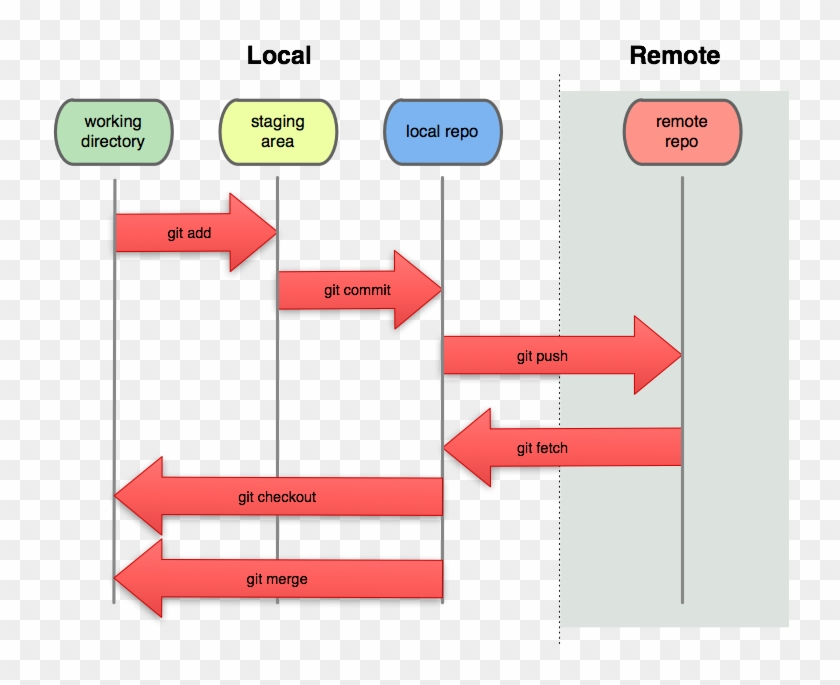
\includegraphics[width=0.8\textwidth]{images/tecnologie/comandi_git.png}
    \caption{Comandi di base di Git}
    \label{fig:git_workflow}
\end{figure}
Essenzialmente un workflow di base con \textbf{Git} prevede:
\begin{list}{-}{}
    \item \textbf{Clonare} un \gls{repository}{}, se già esistente;
    \item \textbf{Modificare} i file all'interno della \gls{working directory}{};
    \item \textbf{Stage} dei file, ovvero prepararli per il prossimo \textit{commit}, aggiungendoli alla \textit{staging area} con il comando \textit{git add};
    \item \textbf{Commit} dei file, ovvero versionarli, con il comando \textit{git commit}, i file così come son salvati nella \textit{staging area} vengono versionati all'interno del \gls{repository}{};
    \item \textbf{Push} delle modifiche sul \gls{repository}{} remoto.
\end{list}
\subsubsection{GitHub}
Per quanto riguarda il servizio di hosting che ha ospita il \gls{repository}{} remoto è stato utilizzato \textbf{GitHub}, andando a condividere 
i contenuti tra il mio account e quello del tutor aziendale (Figura \ref{fig:github}).\\
\begin{figure}[h]
    \centering
    
\includegraphics[width=0.4\textwidth]{images/tecnologie/logo_github.png}
    \caption{Logo di GitHub}
    \label{fig:github}
\end{figure}
\\
\textbf{GitHub} è una piattaforma di hosting per progetti software, che utilizza \textbf{Git} come sistema di controllo di versione e contiene tutti 
i file e i \gls{metadati}{} relativi alle modifiche validate lungo le fasi del progetto.\\
\pagebreak
\subsection{Documentazione}
Per quanto riguarda la redazione della documentazione, Sync Lab non ha uno standard prefissato e mi ha permesso di scegliere quale software utilizzare per la 
produzione dei documenti. La scelta è ricaduta su \textbf{LaTeX}, un linguaggio di markup per la preparazione di testi.\\
\subsubsection{LaTeX}
\textbf{LaTex}  è un sistema di composizione tipografica ampiamente utilizzato per la creazione di documenti di alta qualità. A differenza dei tradizionali editor di testo, LaTeX si basa su comandi di formattazione e struttura, consentendo agli utenti di concentrarsi sul contenuto del documento anziché sul suo aspetto visivo.\\
È stato sviluppato da Leslie Lamport negli anni '80 come estensione di TeX, un linguaggio e motore di composizione sviluppati da Donald Knuth (Figura \ref{fig:latex}).

\noindent \textbf{LaTeX} semplifica notevolmente la creazione di documenti complessi, grazie alla sua capacità di gestire automaticamente numerazione delle sezioni, citazioni bibliografiche, tabelle dei contenuti e molte altre funzionalità tipografiche avanzate.
L'ecosistema che \textbf{LaTeX} offre una vasta gamma di pacchetti e stili predefiniti che consentono di creare documenti sofisticati e professionali.
Per quanto riguarda la scelta dell'editor da utilizzare l'azienda non ha dato vincoli rilevanti, quindi la scelta è ricaduta su \textbf{TexLive}, un distribuzione \textbf{LaTeX} per sistemi operativi Linux e su \textbf{Texworks} come editor di testo.
\begin{figure}[h]
    \centering
    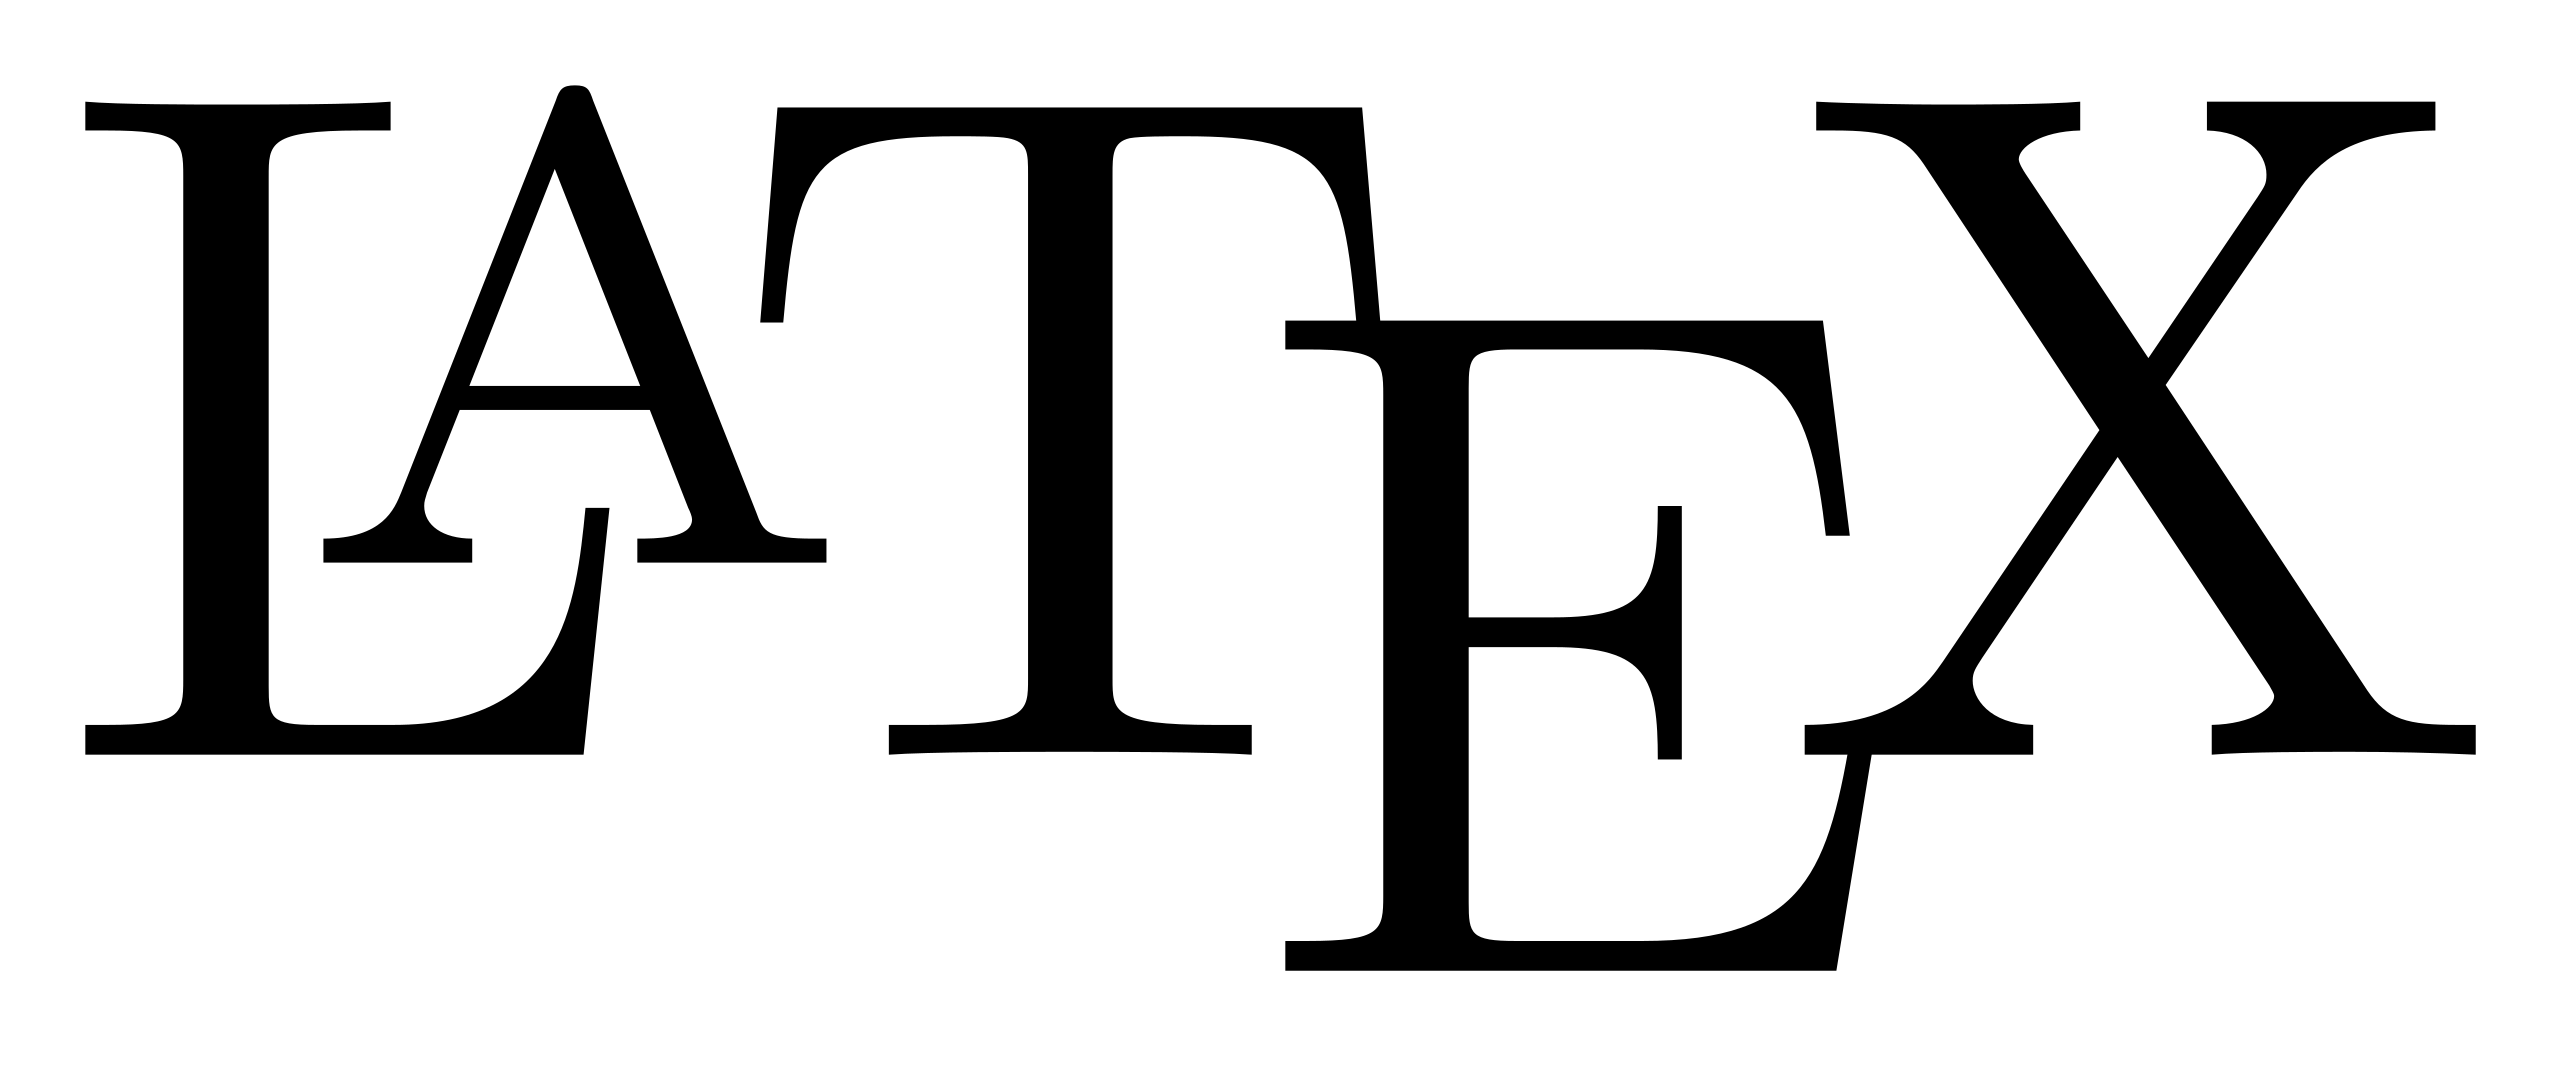
\includegraphics[width=0.3\textwidth]{images/tecnologie/logo_latex.png}
    \caption{Logo di LaTeX}
    \label{fig:latex}
\end{figure}
\subsection{Vincoli implementativi}
Per quanto riguarda l'implementazione del prototipo richiesto dall'azienda, non sono stati dati particolari vincoli implementativi,
se non che il prodotto finale debba essere eseguibile con Docker Compose e che metta in evidenza l'architettura richiesta. 
\newpage
\pagestyle{empty}
\null % o \mbox{} o \phantom{X}
\newpage
    \pagebreak
    \chapter{Componenti di una Data Pipeline}\label{cap:Componenti di una Data Pipeline}
\section{Apache Kafka}
\subsection{Introduzione}
\textbf{Apache Kafka} è una piattaforma \gls{open source}{}, da Jay Kreps, Neha Narkhede e Jun Rao presso LinkedIn e successivamente donata alla \gls{Apache Software Foundation}{} nel 2011. (Figura \ref{fig:logo_kafka}).\\
\textbf{Apache Kafka} nasce con la necessità di LinkedIn di gestire grandi quantità di dati in tempo reale.\\ Già nel 2007 
Jay Kreps e il suo team si resero conto che le soluzioni allora attuali, basate su database tradizionali, non erano in grado di gestire 
un carico di lavoro crescente e la complessità del formato dei dati generati da LinkedIn.\\
Dunque per affrontare tale sfida, nel 2010 LinkedIn iniziò a utilizzare \textbf{Apache Kafka} per gestire i dati di log generati dai vari servizi. \\
Tale adozione ha dimostrato nel tempo che \textbf{Apache Kafka} è in grado di gestire carichi di lavoro molto elevati, di scalare facilmente e di garantire un elevato livello di affidabilità nella consegna di messaggi.\\ 
\textbf{Kafka} è sviluppato in Java e Scala e rilasciata sotto licenza Apache 2.0. La versione attuale è la 3.5.1 rilasciata il 21 luglio 2023.\\
\textbf{Kafka} nasce originariamente come \gls{message broker}{} e permette di gestire uno \gls{streaming di eventi}{} in tempo reale. \\ 
In particolare fornisce funzionalità per:
\begin{list}{*}{}
    \item pubblicare e sottoscrivere flussi di eventi, importandoli ed esportandoli da altri sistemi;
    \item archiviare tali flussi in modo affidabile e duraturo;
    \item elabora flussi di eventi in real time o in modo retrospettivo.
\end{list}
\begin{figure}[h]
    \centering
    
\includegraphics[width=0.5\textwidth]{images/componenti/logo_kafka.png}
    \caption{Logo di Apache Kafka}
    \label{fig:logo_kafka}
\end{figure}
\pagebreak
\subsection{Casi d'uso}
\textbf{Apache Kafka} viene ampliamente utilizzato in tutti quelli scenari in cui è richiesto la gestione 
affidabile di grandi quantità di dati in tempo reale.\\
I principali campi di utilizzo di \textbf{Apache Kafka} sono:
\begin{list}{*}
    \item \textbf{messagistica}: \textbf{Apache Kafka} viene particolarmente utilizzato come \gls{message broker}{}, in applicazioni di messaggistica 
    per disaccoppiare la produzione del messaggio dall'elaborazione dello stesso, \textbf{Kafka} rispetto ai tradizionali \gls{message broker}{} offre velocità e \gls{fault tolerance}{};
    \item \item \textbf{elaborazione del flusso dati}: è possibile anche utilizzare \textbf{Kafka} come componente principale per creare \gls{Data Pipeline}{} in cui i dati grezzi,
    provenienti da diverse sorgenti \textbf{Kafka} vengono aggregati, trasformati fino a ottenere un dato elaborato;
    \item \textbf{monitoraggio e analisi}: \textbf{Kafka} può essere utilizzato per raccogliere dati di monitoraggio provenienti da applicazioni, sistemi di controllo o siti web; 
    \item \textbf{archiviazione dei dati}: \textbf{Apache Kafka} può essere utilizzato come sistema di archiviazione dei dati a lungo termine, permettendo così analisi storiche e ripristino di sistemi 
    in caso di guasti;

\end{list}
\subsection{Architettura e funzionamento}
\textbf{Apache Kafka} nasce come sistema distribuito che opera su nodi (Figure \ref{fig:kafka_architecture}), i quali comunicano tramite protocollo o tramite protocollo
\gls{tcp}{} ad alte prestazioni.Data la sua natura distribuita implementa funzionalità di \gls{fault tolerance}{} con possibilità di rimpiazzo dei nodi che hanno avuto un malfunzionamento.\\  
\textbf{Kafka} può essere distribuito e utilizzato in vari modi tra cui \gls{virtual machine}{} e \gls{container}{}, \gls{on-promise}{}, o servizi cloud.\\
In generale \textbf{Apache Kafka} e costituito da due componenti essenziali: server e client.
\subsubsection{server}
\textbf{Kafka} viene eseguito come un cluster di uno o più server, che rivestono diversi ruoli. \\Alcuni svolgono la funzione di \textbf{Kafka Broker}: ricevono i messaggi dai produttori, li archiviano e inviano i messaggi ai rispettivi consumatori, al momento della sottoscrizione.
\\ Altri invece assolvono il compito di \textbf{Kafka Connect}: importano ed esportano i
dati sotto forma di flussi dati, permettendo così  d'interagire con altri sistemi esistenti.
\subsubsection{client}
I \textbf{client} sono un insieme di librerie che consentono di scrivere applicazioni distribuite e microservizi che permettono d'interagire con
il sistema di messaggistica di \textbf{Apache Kafka}, leggendo, scrivendo ed elaborando flussi di messaggi in parallelo, su larga scala e con \gls{fault tolerance}{} anche in caso di
problemi di rete o guasti della macchina.\\
In generale la scelta del client da utilizzare dipende dal linguaggio di programmazione che si vuole utilizzare per sviluppare l'applicazione.
\subsubsection{I replicas}
In \textbf{Apache Kafka} i \textbf{replicas} costituiscono una parte cruciale dell'architettura e permettono di disporre  di più copie dei dati, distribuite su
più \gls{message broker}{}. Tale meccanismo permette di garantire la \gls{fault tolerance}{} e la scalabilità del sistema.\\
Le repliche possono essere utilizzate a livello di partizione. \textbf{Kafka} ne designa una chiamata \textit{Leader}
mentre le altre sono partizioni \textit{follower o in-sync}. Il numero totale di repliche incluso il
leader costituisce \textbf{il fattore di replicazione}. \\
Il leader e responsabile della ricezione e dell’invio
dei dati, per quella partizione, mentre i \textit{follower} ricevono i dati dal leader e li replicano.\\
\subsubsection{Produttori e consumatori}
Il produttore \textbf{Kafka} invia i dati, con una richiesta di deposito,  direttamente al \gls{message broker}{}, \textit{Leader} della partizione. Per velocizzare la ricerca del
\textit{Leader}, tutti i nodi possono rispondere alle richieste dei produttori fornendo \gls{metadati}{} su quali nodi sono presenti i \textit{Leader}, tale informazione consentirà al produttore d'indirizzare in modo
appropriato i messaggi.\\
D'altra parte il consumatore emette una richiesta di recupero di messaggi al \gls{message broker}{} che funge da \textit{Leader} della partizione, specificando il suo offset nel registro dei messaggi.\\
Il \gls{message broker}{} risponde con un messaggio contenente il suo offset nel registro con ogni richiesta e con una parte del registro a partire da quella posizione. \\
Per quanto riguarda l'estrazione e il recupero dei messaggi: i dati vengono inviati al broker dal produttore e prelevati dal \gls{message broker}{} dal consumatore. 
\subsubsection{La struttura dei messaggi}
I messaggi inviati all'interno di \textbf{Apache Kafka} sono composti da una chiave, un valore e un timestamp. \\
Oltre a tali informazioni a ogni messaggio viene associato un \gls{topic}{} o argomento che permette di eseguire operazioni di organizzazione 
e filtraggio dei messaggi.\\
Un messaggio, una volta inviato a un consumatore non viene eliminato dal \gls{topic}{} ma viene mantenuto per un periodo di tempo configurabile attraverso un timeout.\\
I \gls{topic}{} dei rispettivi messaggi vengono partizionati su più nodi per consentire a più consumatori di leggere gli stessi messaggi e permettendo ai client di leggere e scrivere messaggi da/a molti \gls{message broker}{}.\\
Quando un nuovo messaggio viene emesso, quest'ultimo si aggiunge alla rispettiva partizione relativa al \gls{topic}{} e viene assegnato un numero di offset che identifica il messaggio all'interno della partizione.\\
Grazie a tale meccanismo \textbf{Apache Kafka} garantisce che i messaggi vengano letti nell'ordine in cui sono stati scritti.
\subsubsection{Zookeeper}
\textbf{Zookeeper} è un prodotto \gls{open source}{} che si occupa della sincronizzazione tra i cluster distribuiti di sistemi come \textbf{Apache Kafka}. \\
È progettato per gestire operazioni di sincronizzazione, gestione dello stato e configurazioni nei sistemi distribuiti, garantendo coerenza e affidabilità.\\
Il suo funzionamento si basa sul protocollo Zookeeper Atomic Broadcast (ZAB), che è il cuore del servizio di coordinamento di \textbf{Zookeeper}.\\
Ogni nodo invia a intervalli regolari un messaggio \textit{Keep-Alive} a \textbf{Zookeeper}, informandolo così che è vivo e funzionante. Se entro un tempo prestabilito il messaggio non viene ricevuto si presume che il nodo sia
morto e se era un leader se ne elegge un altro.\\
Inoltre \textbf{Zookeeper} permette di definire dei parametri che consentono di capire quando un nodo è guasto e quanto gli altri nodi, appartenenti a una partizione,  sono in ritardo rispetto al \textit{Leader} in termini di sincronizzazione sull'arrivo dei messaggi.\\
Il parametro \textit{zookeeper.session.timeout.ms}, impostato a 6000 millisecondi per impostazione predefinita, indica che, se il leader non riceve l'evento \textit{Keep-Alive} entro quel periodo temporale, detiene che quel nodo sia guasto.\\
Il parametro \textit{replica.lag.max.messages}, indica la massima differenza consentita tra \textbf{Replica's Offset}e \textbf{Leader's Offset}. Se tale differenza è maggiore di \textit{replica.lag.max.message-1}, il nodo viene considerato in ritardo e viene rimosso dall'elenco dei nodi in sincronizzazione dal leader. \\
Tutti i nodi che sono attivi e sincronizzati formano l' \textbf{In-Sync Replica Set}(\textbf{ISR}).\\
Se tutti i nodi in sincronizzazione hanno memorizzato un messaggio nei rispettivi \gls{log}{}, questo messaggio viene considerato confermato e quindi inviato ai consumatori. \\
In questo modo, un sistema come \textbf{Kafka} garantisce che un messaggio di cui è stato eseguito il \textit{commit} non andrà perso, purché sia presente almeno una replica attiva e sincronizzata, in ogni momento.\\
Un nodo non sincronizzato può ricongiungersi all'\textbf{ISR} se può sincronizzarsi completamente di nuovo, anche se ha perso alcuni dati a causa del suo arresto anomalo.
\subsubsection{Politiche di retentions}
Con \textbf{Retention} in \textbf{Kafka} si intende la possibilità di controllare la dimensione dei registri
degli argomenti ed evitare di superare le dimensioni del disco esistente.\\
La conservazione può essere configurata o controllata in base alla dimensione dei \gls{log}{} o in
base alla durata configurata. Tale configurazione può essere impostata a grana fine o a
grana grossa per ogni argomento o per tutti gli argomenti.
\paragraph{Retention basata sulle dimensione}
Una volta raggiunto il tempo di conservazione configurato per il segmento, quest'ultimo viene contrassegnato per l'eliminazione o la \gls{compattazione}{} in base al criterio di pulizia configurato. Il periodo di conservazione predefinito per i segmenti è di 7 giorni.
I parametri configurabili per la \textbf{Retention} basata sul tempo sono in ordine d'importanza e valutazione sono:
\begin{enumerate}
    \item $log.retention.ms$;
    \item $log.retention.minutes$;
    \item $log.retention.hours$.
\end{enumerate}
Nel momento in cui un parametro di livello di priorità superiore non è impostato si segue la politica di conservazione del parametro di livello di priorità inferiore.\\
\paragraph{Retention basata sulla dimensione}
In questo caso si va configurare la dimensione massima di una struttura di dati di registro per una partizione di argomento. Una volta che la dimensione del registro raggiunge questa dimensione, inizia a rimuovere i segmenti dalla sua fine.\\

I parametri configurabili per la \textbf{Retention} basata dimensione sono in ordine d'importanza e valutazione:
\begin{enumerate}
    \item $log.segment.bytes$: la dimensione massima di un singolo file di registro;
    \item $log.retention.check.interval.ms$: la frequenza in millisecondi con cui la pulizia del registro verifica se un registro è idoneo per l'eliminazione;
    \item $log.segment.delete.delay.ms$: la quantità di tempo da attendere prima di eliminare un file dal file system.
\end{enumerate}


\begin{figure}[h]
    \centering
    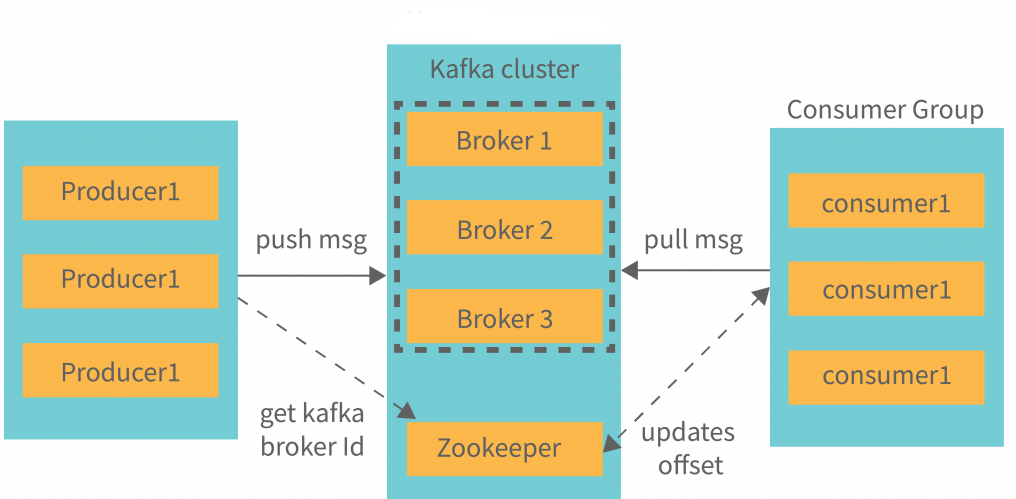
\includegraphics[width=0.9\textwidth]{images/componenti/kafka_architetcture.png}
    \caption{Architettura di Apache Kafka}
    \label{fig:kafka_architecture}
\end{figure}

\subsection{Garanzie di funzionamento}
In \textbf{Kafka} esistono produttori e consumatori che producono e sottoscrivono eventi. Gli uni, essendo in un ambiente distribuito,
sono indipendenti l’uno dall’altro. \\
\textbf{Apache Kafka} in tale contesto può fornire una delle seguenti garanzie sulla consegna e ricezione dei messaggi:
\begin{list}{*}
    \item \textbf{at most once}: i messaggi vengono consegnati al consumatore al più una volta. In questo caso, i messaggi possono essere persi, ma non duplicati;
   \item \item  \textbf{at least once}: i messaggi vengono consegnati al consumatore almeno una volta, i messaggi possono essere duplicati, ma non persi;
    \item \textbf{exactly once}: i messaggi vengono consegnati al consumatore esattamente una volta. In questo caso, i messaggi non vengono né persi né duplicati, è la garanzia più costosa ma maggiormente richiesta.
\end{list}
\subsection{Il pattern Publisher-Subscriber}
\textbf{Apache Kafka}, nell'elaborazione dei messaggi, implementa il pattern \textbf{Publisher-Subscriber} (Figura \ref{fig:publisher_subscriber}) che permette di gestire flussi di dati in tempo reale.\\
Il pattern architetturale \textbf{Publisher-Subscriber} è un modello di progettazione software, utilizzato nei sistemi distribuiti, che impiegano una comunicazione asincrona tra i vari componenti.\\
Sebbene vada ad utilizare tecniche già preesistenti come la sottoscrizione e l'accodamento di messaggi, la  chiave di successo di tale pattern è il totale disaccoppiamento delle componenti: i componenti non sono a conoscenza dell'identità e della presenza degli altri.\\
Tale modello è nato dalla necessità del rendere i sistemi ridimensionabili in modo dinamico. Per raggiungere tale obiettivo, lo scambio di messaggi 
tra i due agenti in gioco viene gestito da un intermediario, chiamato \textbf{broker}, che si occupa di ricevere i messaggi dai \textbf{publisher} e di inoltrarli ai \textbf{subscriber}.\\
\subsubsection{Vantaggi}
\begin{itemize}
    \item \textbf{Debole accopiamento tra le componenti}:  rende il sistema più flessibile e modificabile dinamicamente;
    \item \textbf{Elevata scalabilità}: non esiste limite al numero di \textbf{publisher} e \textbf{subscriber} che possano comunicare;
    \item \textbf{Utilizzo della comunicazione ascincrona ad eventi}: non necessità della sincrona degli attori coinvolti nella comunicazione;
    \item \textbf{Indipendente dal protocollo di comunicazione}: è integrabile con qualsiasi protocollo di comunicazione e stack tecnologico.
\end{itemize}
\begin{figure}[h]
    \centering
    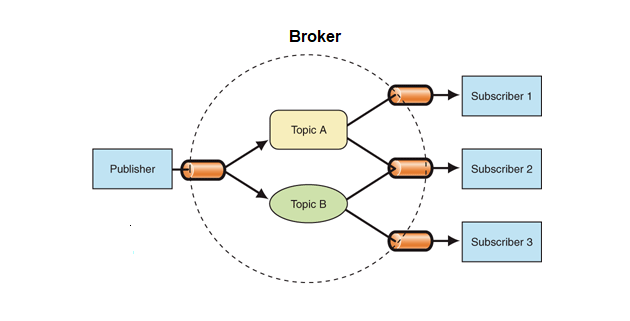
\includegraphics[width=0.9\textwidth]{images/componenti/ps-model.png}
    \caption{Il pattern Publisher-Subscriber}
    \label{fig:publisher_subscriber}
\end{figure}
\pagebreak
\subsection{Even Driven Architecture}
L'\textbf{Even Driven Architecture} è un pattern architetturale basato su eventi: degli agenti, che sono in grado di ricevere tali eventi, agiscono solo nel momento in cui questi ultimi si verificheranno. 
\\Una architettura basato su eventi fornisce una serie di altri vantaggi basati sul disaccoppiamento tra il produttore e il consumatore dell'evento, i quali, nel momento dell'emissione di quest'ultimo non è necessario siano sincroni ma possono andare a sfruttare una comunicazione di tipo asincrona. 
\subsubsection{Apache Kafka e l'architettura EDA}
L'emissione di un evento indica che qualcosa è accaduto e può essere visto come un agglomerato di dati atomico in grado di soddisfare l'evento stesso. \\
Di solito \textbf{Apache Kafka} viene descritto anche come una piattaforma di \gls{streaming di eventi}{} gestisti come flusso continuo di dati. \\Inoltre \textbf{Kafka} memorizza tali dati in modo duraturo per il successivo recupero, analisi o elaborazione in tempo reale.
\\D'altra parte per utilizzare \textbf{Kafka} in un sistema \textbf{EDA} la chiave è andare a sfruttare il disaccopiamento: invece di effettuare un polling continuo di verifica della presenza di nuovi dati, basterà ascoltare il verificarsi di un evento per agire di conseguenza. Inoltre grazie all'approcio sviluppato da \textbf{Kafka} un evento una volta soddisfatto non viene eliminato, ma conservato per un periodo ti tempo predeterminato, pertanto un evento potrà essere letto da più consumatori e potrà essere utilizzato per soddisfare una varietà di richieste, fino alla scadenza del suo periodo di conservazione. \\
\pagebreak
\section{Apache Druid}
\textbf{Apache Druid} (Figura \ref{fig:logo_druid}) è uno strumento \gls{open source}{} di analisi \gls{olap}{} progettato per analizzare e gestire grandi moli di dati in tempo reale, in modo scalabile. \\
Il progetto su cui si basa \textbf{Apache Druid} è stato sviluppato a partire dal 2011 da Metamarkets, una società di analisi dei dati in tempo reale per il settore pubblicitario,
da parte di Gian Merlino, Eric Tschetter e Fangjin Yang.\\
L'obiettivo iniziale era quello di creare un sistema in grado di analizzare, in tempo reale, grandi quantità di dati per fornire ai clienti 
informazioni sulle campagne pubblicitarie.\\
Purtroppo le tecnologie allora esistenti non erano in grado di soddisfare le esigenze di Metamarkets, pertanto il team di sviluppo decise di creare un nuovo sistema che potesse soddisfare le loro esigenze, che ha preso il nome di \textbf{Druid}.\\
\textbf{Druid} nasce per gestire dati di tipo evento, come strumento di \gls{log}{}, dati di transazione e molti altri. \\
Nel 2012, Metamarkets ha rilasciato \textbf{Druid}{} come progetto \gls{open source}{} su GitHub, permettendo così alla comunità di contribuire e sviluppare ulteriormente la piattaforma. Nel 2015, \textbf{Druid} è diventato un progetto \gls{open source}{} ufficiale sotto l'autorità della \gls{Apache Software Foundation}{}.\\ 
\textbf{Apache Druid} è comunemente utilizzato come back-end per le GUI di applicazioni analitiche o
per \gls{api}{} altamente simultanee che richiedono aggregazioni veloci. \\
\textbf{Druid} è sviluppato in Java e Scala, rilasciato sotto licenza Apache 2.0. \\La versione attuale è la 27.0.0 rilasciata il 10 agosto 2023.\\
\begin{figure}[h]
    \centering
    
\includegraphics[width=0.5\textwidth]{images/componenti/logo_druid.png}
    \caption{Logo di Apache Druid}
    \label{fig:logo_druid}
\end{figure}
\subsection{Casi d'uso}
\textbf{Apache Druid} viene utilizzato in tutti quegli scenari in cui è necessario analizzare grandi quantità di dati in tempo reale, in modo scalabile, con \gls{fault tolerance}{} e con la possibilità di effettuare query complesse ad alta efficienza.\\  
I principali campi di utilizzo di \textbf{Apache Druid} sono:
\begin{list}{*}
    \item \textbf{analisi dati in real-time e applicazioni dati}: \textbf{Apache Druid} viene ampliamente impiegato sistemi di acquisizione dati in
    tempo reale, query rapide e tempo di attività. \textbf{Druid} viene utilizzato per alimentare GUI
    di applicazioni analitiche o per \gls{api}{} simultanee che necessitano di aggregazioni veloci, i migliori risultati 
    vengono ottenuti nell'analisi di dati di tipo evento;
    \pagebreak
    \item \item \textbf{elaborazione di metriche}: \textbf{Apache Druid} viene spesso utilizzato per effettuare misurazioni sul coinvolgimento degli
    utenti e il monitoraggio dei dati di test, calcolando metriche, conteggi finalizzati a elaborare tendenze su grandi moli di dati;
    \item \textbf{operazioni \gls{olap}{}}: \textbf{Apache Druid} viene utilizzato per accelerare l’esecuzione di query su grandi moli di dati e potenziare le applicazioni; è progettato per un’elevata concorrenza e query in meno di un secondo, alimentando
    l’esplorazione interattiva dei dati attraverso un’interfaccia utente.
\end{list}
\subsection{Architettura e funzionamento}
\textbf{Apache Druid} include molteplici configurazione sia su singolo nodo, che distribuito su un \gls{cluster}{}.\\
Le distribuzioni su singolo nodo sono ormai poco utilizzate, ma esistono altre configurazioni pensate per macchine con bassa disponibilità di 
CPU e memoria, pensate appositamente piccoli \gls{container}{} \gls{Docker}{}. 
\subsubsection{Distribuzione su cluster}
\textbf{Apache Druid} nasce come sistema distribuito, scalabile, tollerante ai guasti, compatibile con il cloud. \\
Inoltre una architettura di questo tipo un malfunzionamento di una componente non influisce immediatamente sulle altre.\\

In generale un \gls{cluster}{} di \textbf{Apache Druid} ospita i seguenti server: 
\begin{list}{*}
    \item \textbf{i server principali}: sono responsabili della gestione dei \gls{metadati}{} e delle esigenze di coordinamento del \gls{cluster}{}, possono essere collocati insieme sullo stesso server;
    \item \item \textbf{i server dati}: finalizzati a  gestire i dati effettivi all'interno \gls{cluster}{}, traggono grandi vantaggi da CPU, RAM e SSD;
    \item  \textbf{i server d'interrogazione}: chiamati anche \textbf{Druid Broker}, accettano le richieste e le distribuiscono al resto del cluster.
\end{list}
\paragraph{I server principali} o \textbf{Master} gestiscono l’\gls{injection}{} e la disponibilità dei dati: sono i responsabile dell’avvio
di nuovi operazioni di \gls{injection}{} e del coordinamento della disponibilità dei dati sui \textbf{Data server}.\\
Ogni server mantiene una connessione con a un \textbf{Zookeeper} per le informazioni sul \gls{cluster}{} corrente.
I server \textbf{Master} sono formati da:
\subparagraph{I Coordinator} hanno il compito di gestire la disponibilità dei dati dei \gls{cluster}{}, comunicano
agli \textbf{Historical} di caricare o rilasciare segmenti in base alle configurazioni, sono i 
responsabili del caricamento di nuovi segmenti, dell’eliminazione di segmenti obsoleti, della
garanzia che i segmenti siano replicati (caricati su piu nodi \textbf{Historical} diversi) un
numero corretto  di volte e sia presente un bilanciamento dei segmenti
tra \textbf{Historical} per mantenere quest’ultimo caricato uniformemente.Il \textbf{Coordinator} ha anche una connessione a un database
contenente l’elenco dei segmenti utilizzati. 
\subparagraph{Gli Overlord} sono i responsabili dell’accettazione delle attività, del coordinamento della distribuzione delle
attività, della restituzione degli stati ai
chiamanti. Possono essere eseguiti sia in modalità locale che su server dedicato. Gli \textbf{Overlord} hanno anche il compito di 
creare i \textbf{Peons} per l'esecuzione delle attività. 
\paragraph{I Server dati} eseguono le attività d'acquisizione e archiviazione dei dati interrogabili.
I server \textbf{dati} sono formati da:
\subparagraph{I server Historical}
\subparagraph{I server MiddleManager} 
\subparagraph{I server Peon}
\paragraph{I Server d'interrogazione} o server \textbf{query} forniscono la funzionalità d'interazione con gli utenti, instradando le richieste  
ai \textbf{server dati} o ad altri \textbf{server query}, per la loro esecuzione. \\
I server \textbf{query} sono formati da:
\subparagraph{I server Broker} sono i server a cui instradare le query, analizzano i \gls{metadati}{} forniti
da \textbf{Zookeeper}, comprendono dove ricavare i dati necessari per elaborare i risultati delle query ed 
infine uniscono tutti i risultati elaborati per fornire un’unica risposta alla richiesta.\\
\subparagraph{I server Router} sono i server che hanno il compito di instradare le query a diversi server \textbf{Broker}. Le query
vengono instradate in base alle regole di caricamento dei segmenti che vengono applicate.
Tale configurazione fornisce l’isolamento delle singole query, anche nel caso in cui si voglia applicare 
una priorità di esecuzione a determinate query.\\
\begin{figure}[h]   
    \centering
    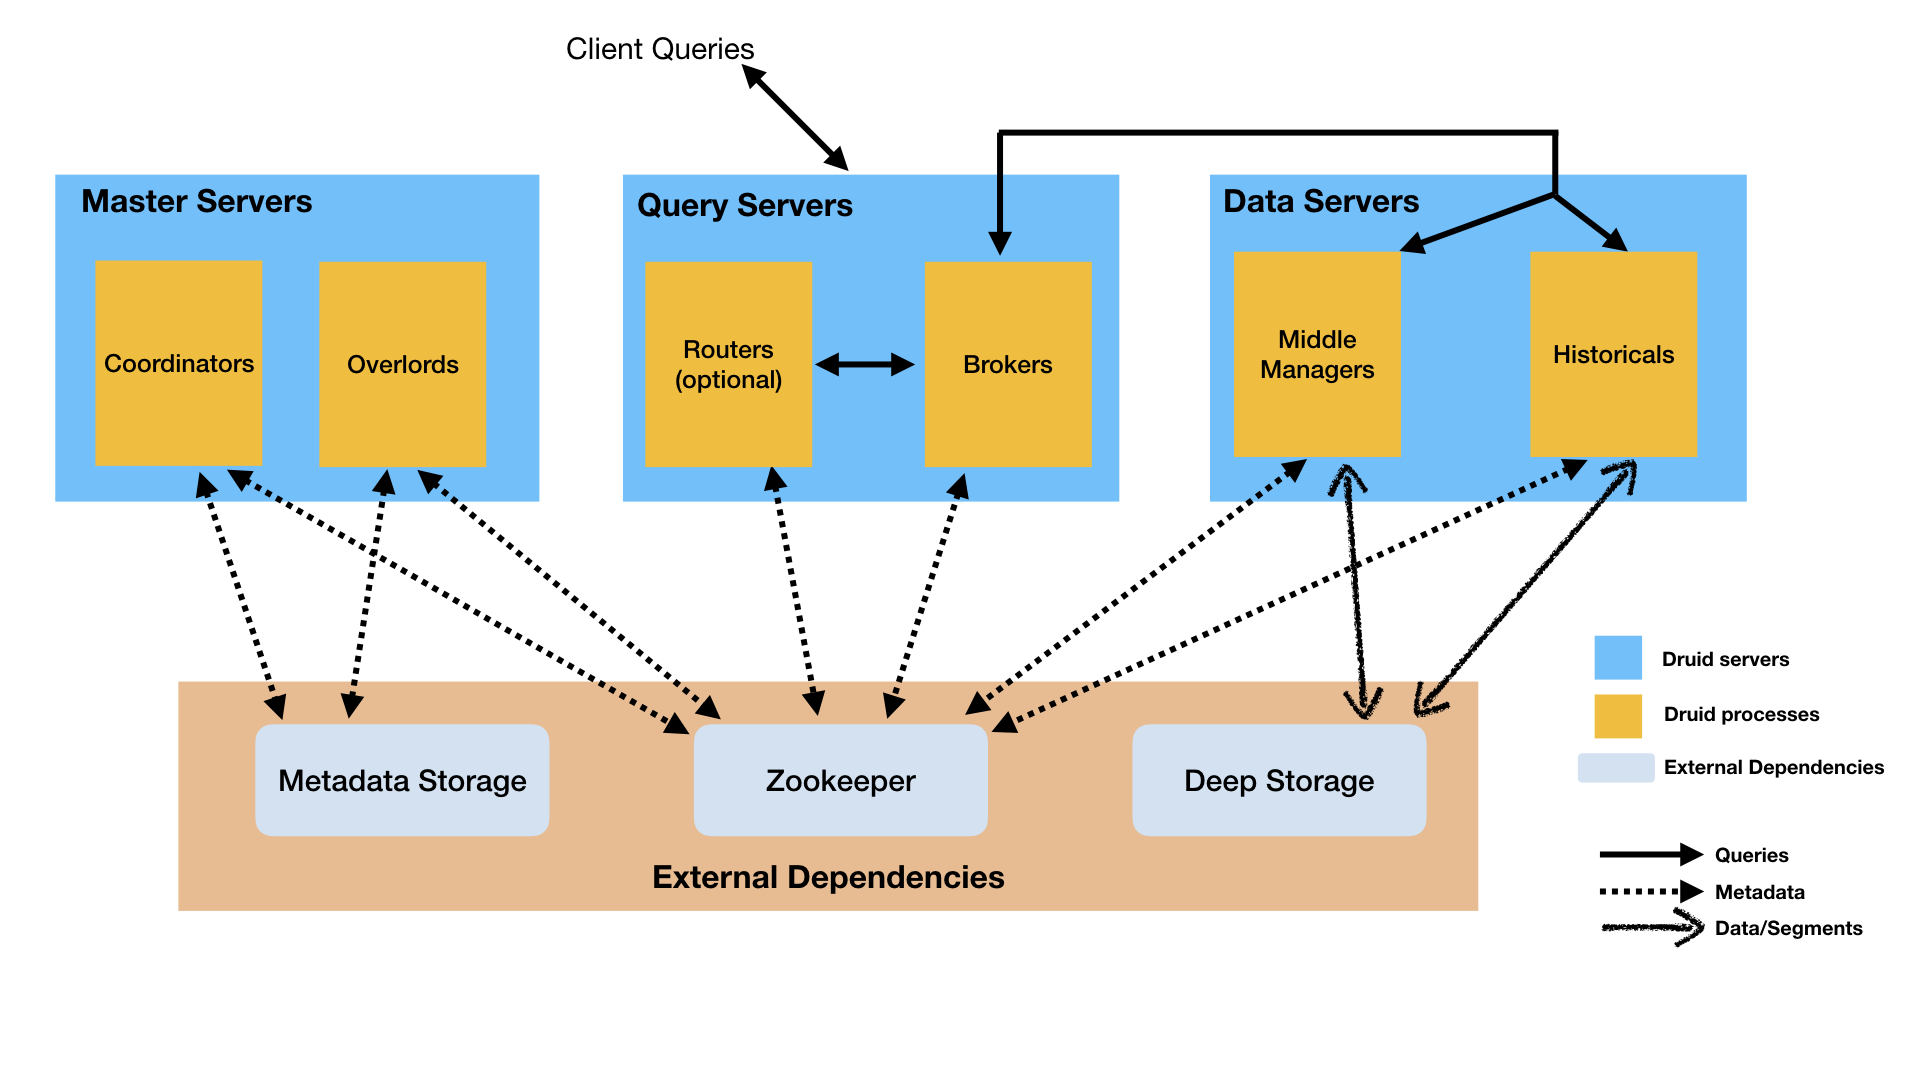
\includegraphics[width=0.9\textwidth]{images/componenti/druid_architectcture.png}
    \caption{Architettura di Apache Druid}
    \label{fig:druid_architecture}
\end{figure}
\pagebreak
\section{Streaming Data Pipelines}
\newpage
\pagestyle{empty}
\null % o \mbox{} o \phantom{X}
\newpage
    \pagebreak
    \chapter{Il percorso di stage }\label{cap:Il_percorso}
\section{Formazione}
Il processo di formazione ha avuto un ruolo fondamentale nella buona riuscita del progetto di stage, con una durata complessiva di circa quattro settimane. \\
La causa del protrarsi del processo di formazione è stata provocata dalla mia inesperienza in merito a 
concetti legati all'architettura \gls{eda}{},
\textbf{Apache Kafka}, \textbf{Apache Druid} e \textbf{Docker Compose}.\\  
Tutto il processo di formazione è stato tracciato e monitorato da me medesimo e dal tutor aziendale attraverso le \gls{board}{} offerte 
dal software di \gls{project management}{} \textbf{ClickUp} (Figura \ref{cap:ClickUp}).\\
\begin{figure}[h]
    \centering
    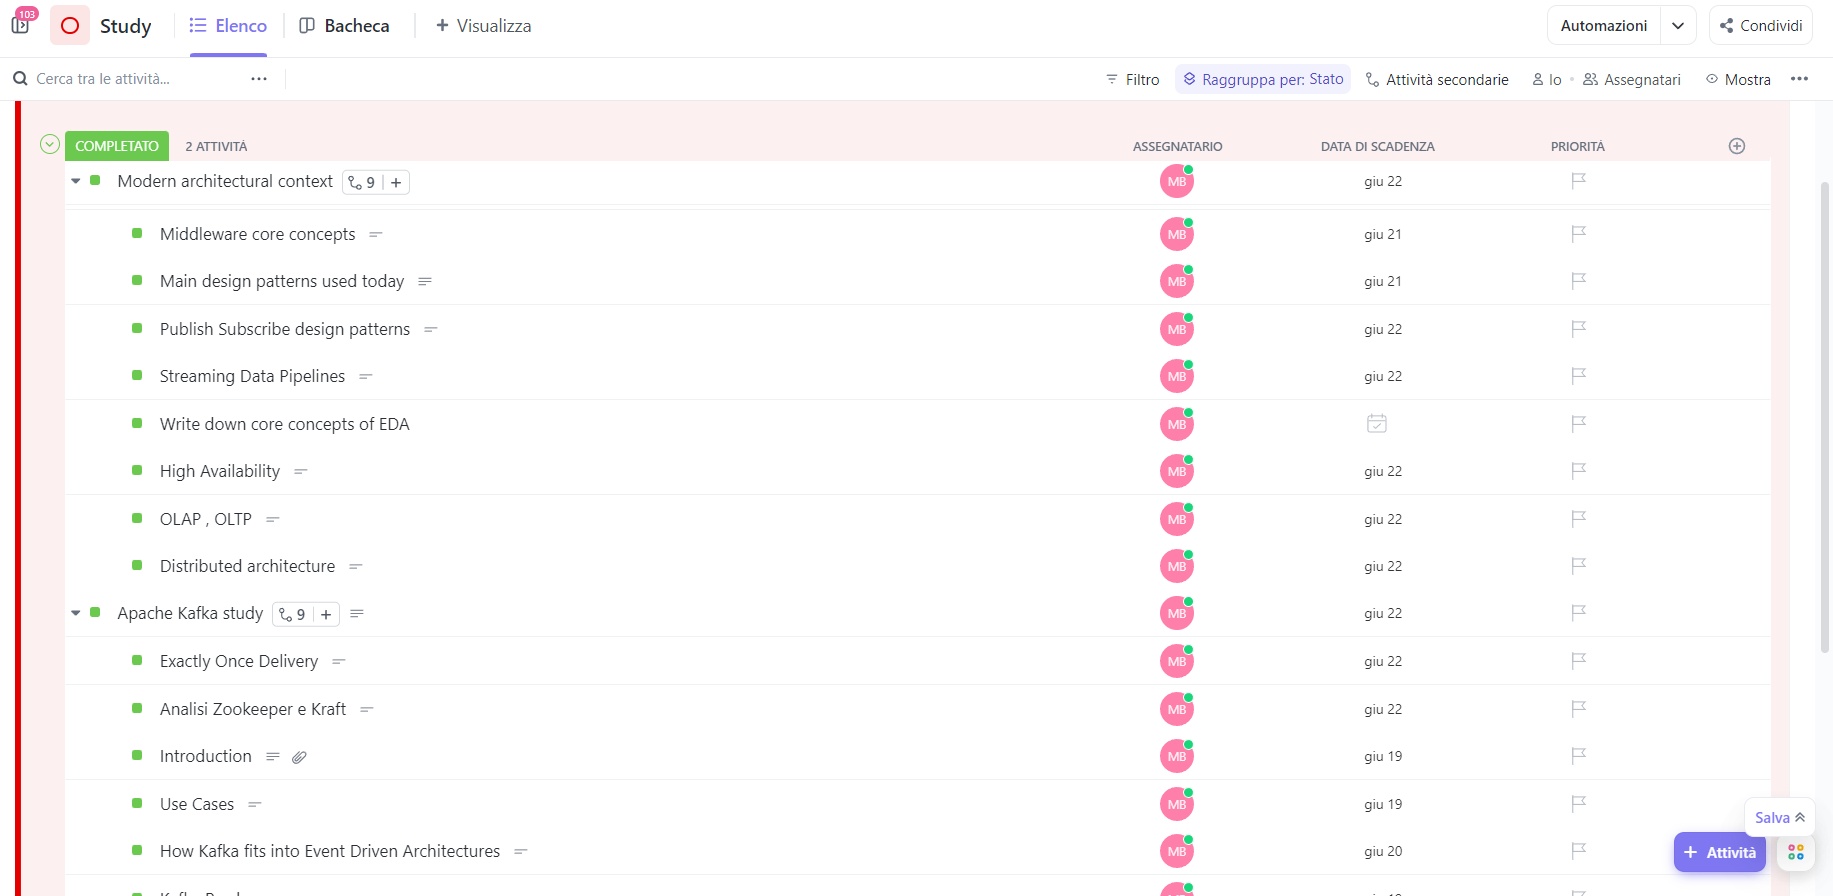
\includegraphics[width=1\textwidth]{images/percorso/formazione.png}
    \caption{Board di ClickUp per il processo di formazione}
    \label{cap:ClickUp}
\end{figure}
\pagebreak
\\
Inoltre durante il processo di formazione, oltre a reperire informazioni da documentazione ufficiale, ho avuto anche modo 
di approfondire quanto appena appreso attraverso delle attività di \gls{hands-on}{} che mi hanno permesso di mettere in pratica nell'immediato quanto appreso
(Figura \ref{cap:Hands-on}).
\begin{figure}[h]
    \centering
    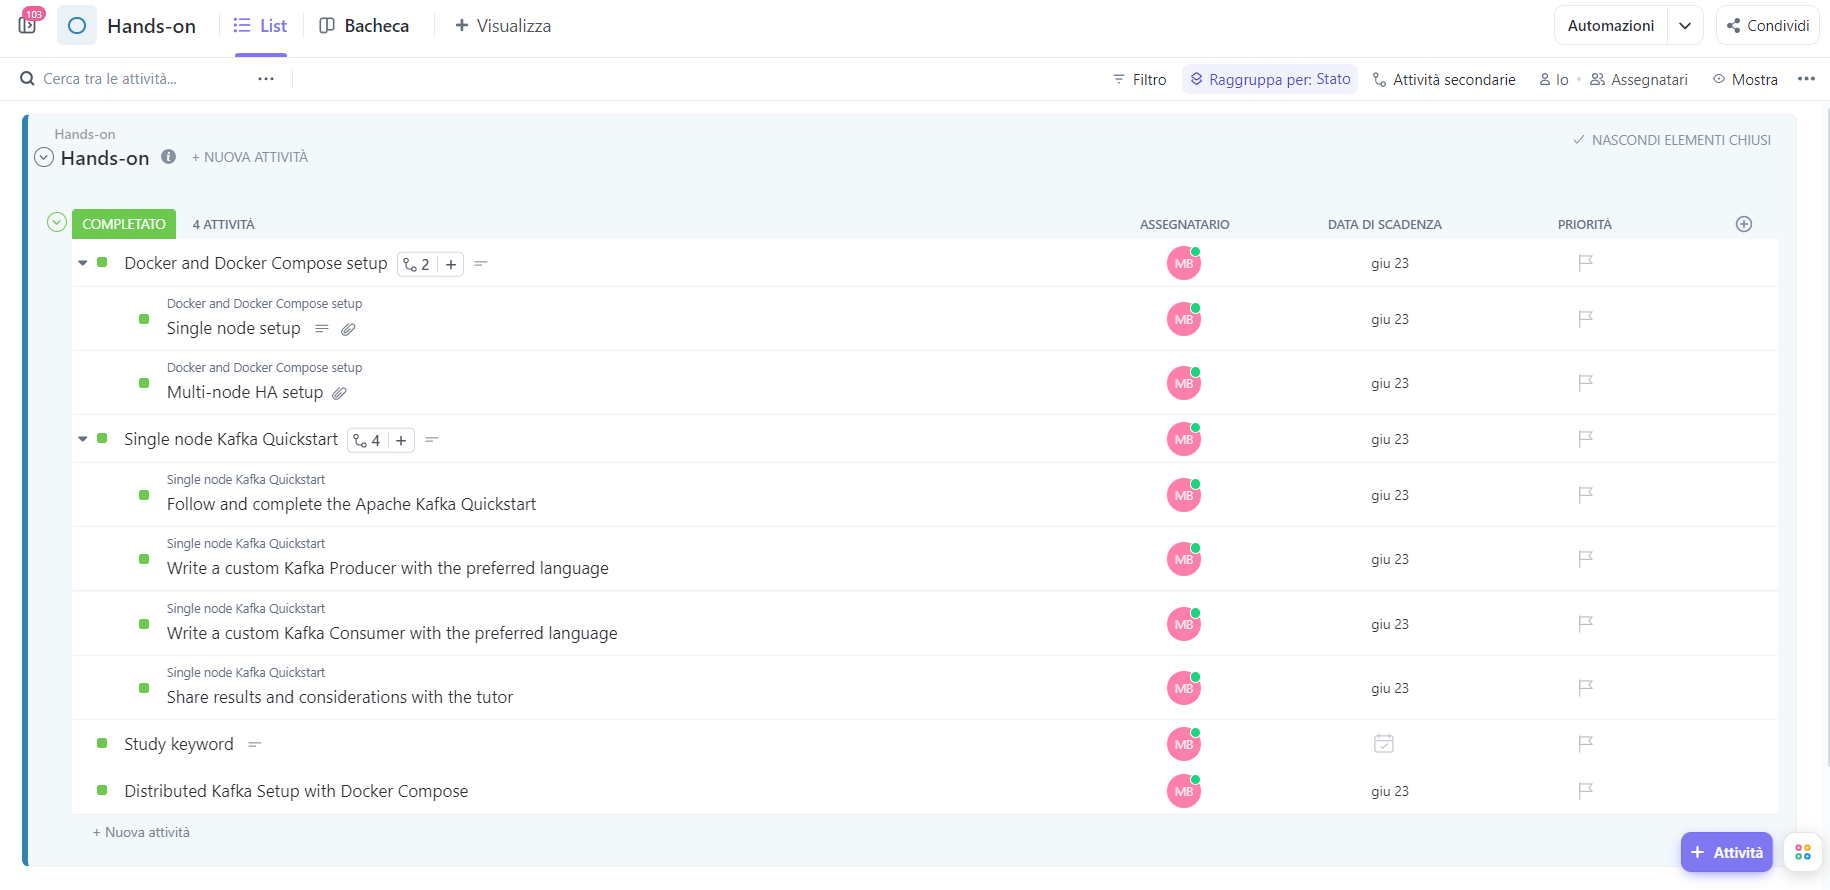
\includegraphics[width=1\textwidth]{images/percorso/hands_on.png}
    \caption{Attività di hands-on per il processo di formazione}
    \label{cap:Hands-on}
\end{figure}
\\
Durante il processo di formazione, in collaborazione con il tutor aziendale, è stato anche definito un processo di coordinamento e produzione di 
documentazione che mi ha permesso, durante tutto lo svolgimento del percorso di stage, di avere un tracciamento dei concetti appresi e 
 di avere un riferimento per un'eventuale risoluzione di problemi o dubbi sorti (Figura \ref{cap:Documentazione}).
\begin{figure}[h]
    \centering
    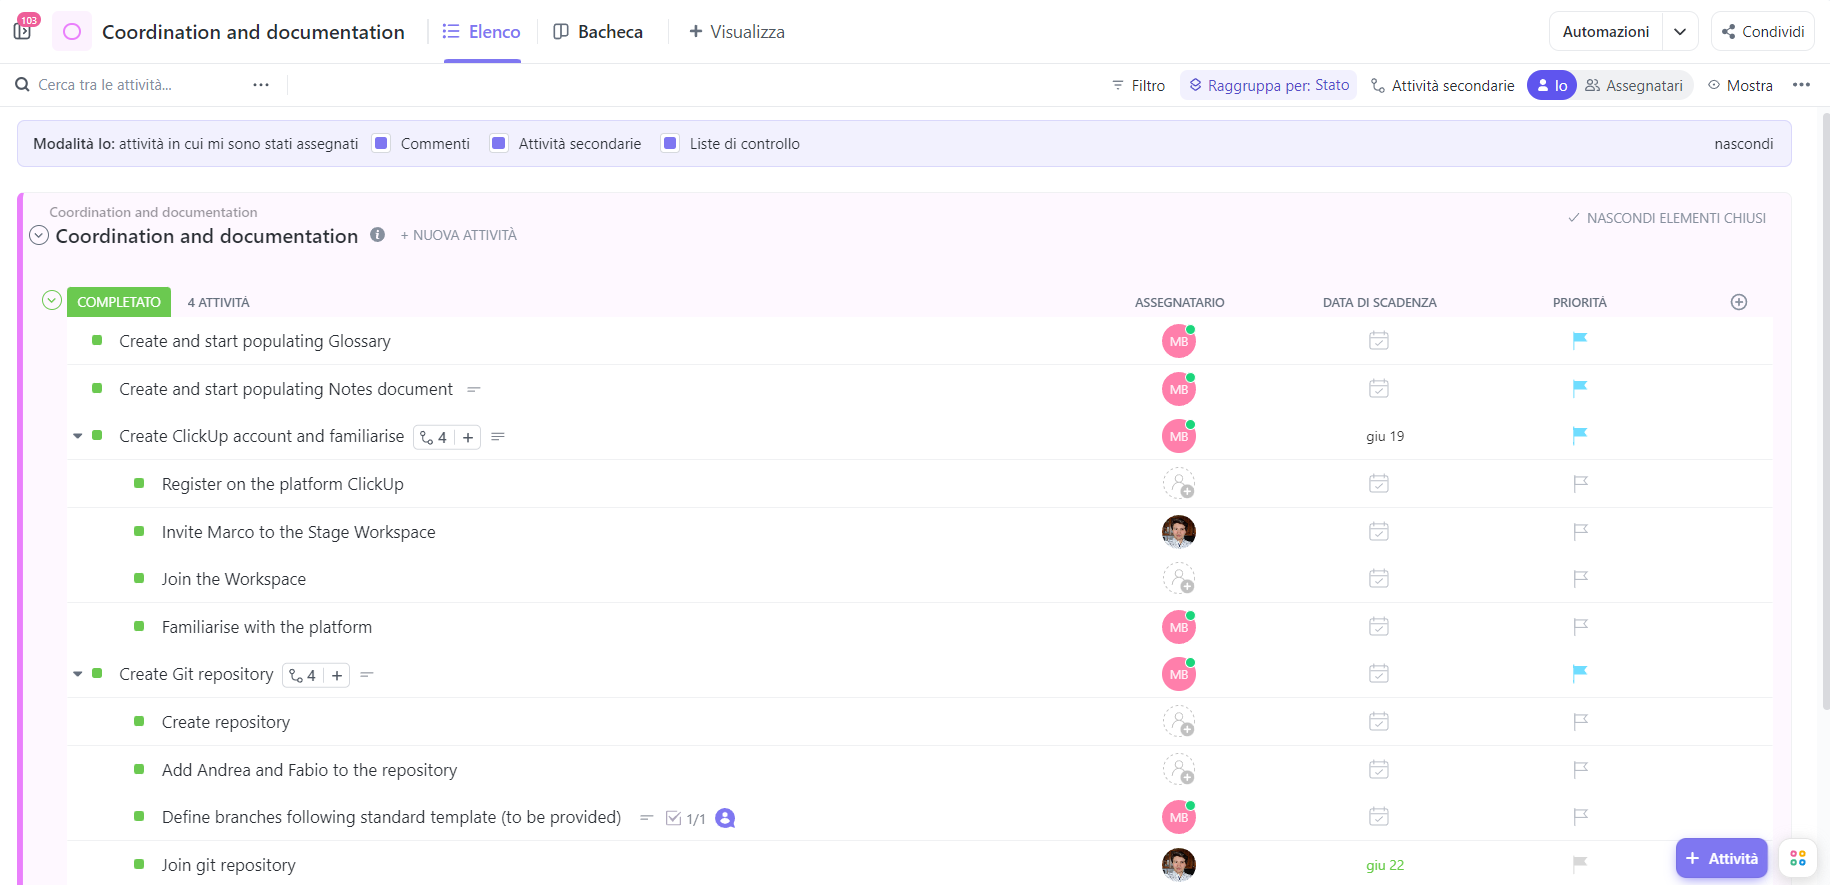
\includegraphics[width=1\textwidth]{images/percorso/coordinamento.png}
    \caption{Board di ClickUp per il processo di coordinamento e documentazione}
    \label{cap:Documentazione}
\end{figure}
\subsection{Daily stand-up meeting}
In ausilio dei processi sopra descritti, 
è stato anche definito, in concomitanza con l'inizio del processo di formazione, un processo di \textbf{supporto} ispirato al metodo \gls{Scrum}{}, 
andando a programmare degli incontri giornalieri di circa 15 minuti finalizzati a:
\begin{list}{*}
    \item \textbf{monitorare} lo stato di avanzamento delle attività svolte, da svolgere e in corso di svolgimento;
    \item \item \textbf{risolvere} eventuali dubbi o problemi sorti durante lo svolgimento delle attività;
    \item \textbf{definire} eventuali miglioramenti o cambiamenti da apportare alle da svolgere, o in corso di svolgimento, e al metodo 
    di lavoro adottato.
\end{list}
\section{Codifica}
\subsection{Configurazione di un cluster Kafka con Docker Compose}
Dopo aver terminato le attività di formazione su \textbf{Apache Kafka} e \textbf{Docker Compose} 
ho iniziato la configurazione di un \gls{cluster}{}, che fa uso di \gls{container}{}, in grado di testare tali strumenti.
\\Seguendo la buona pratica dell'alta affidabilità, descritta del 
paragrafo \ref{sec:alta_affidabilita}, ho configurato un \gls{cluster}{} con tre nodi \textbf{Kafka} e un nodo \textbf{Zookeeper}.\\
Innanzitutto per far che ogni \gls{container}{} possa comunicare con gli altri è stato necessario creare una 
\gls{Docker network}{}, denominata \textbf{kafka-druid}, nel seguente modo.
\begin{lstlisting}[caption=\texttt{docker network create}, label=lst:file]{docker network create}
docker network create kafka-druid
\end{lstlisting}
Successivamente sono stati creati i nodi \textbf{Zookeeper} e \textbf{Kafka} con \textbf{Docker Compose} 
utilizzando il seguente file di 
configurazione (per motivi di spazio viene riportata la definizione di un solo nodo \textbf{Kafka}, la configurazione degli altri è del tutto analoga).
\begin{lstlisting}[caption=\texttt{kafka-cluster-compose.yml}, label=lst:file]{kafka-cluster-compose.yml}
networks:
  kafka-druid:
    name: kafka-druid
    driver: bridge
    external: true
services:
  kafka:
    image: confluentinc/cp-kafka:7.4.0
    hostname: kafka
    container_name: kafka
    networks:
      - kafka-druid
    ports:
      - "29092:29092"
    environment:
      KAFKA_ADVERTISED_LISTENERS: INTERNAL://kafka:9092,EXTERNAL://localhost:29092
      KAFKA_LISTENER_SECURITY_PROTOCOL_MAP: INTERNAL:PLAINTEXT,EXTERNAL:PLAINTEXT
      KAFKA_INTER_BROKER_LISTENER_NAME: INTERNAL
      KAFKA_ZOOKEEPER_CONNECT: "zookeeper:2181"
      KAFKA_BROKER_ID: 1
      KAFKA_LOG4J_LOGGERS: "kafka.controller=INFO,kafka.producer.async.DefaultEventHandler=INFO,state.change.logger=INFO"
      KAFKA_OFFSETS_TOPIC_REPLICATION_FACTOR: 1
      KAFKA_TRANSACTION_STATE_LOG_REPLICATION_FACTOR: 1
      KAFKA_TRANSACTION_STATE_LOG_MIN_ISR: 1
      KAFKA_AUTHORIZER_CLASS_NAME: kafka.security.authorizer.AclAuthorizer
      KAFKA_ALLOW_EVERYONE_IF_NO_ACL_FOUND: "true"

\end{lstlisting}
È importante sottolineare che all'interno della configurazione, sopra descritta, 
vengono utilizzate le \gls{immagini Docker}{} \textbf{confluentinc/cp-zookeeper:7.4.0} e \\\textbf{confluentinc/cp-kafka:7.4.0}.\\
Tale scelta è stata adottata, dal fatto che oramai \textbf{Confluent} 
è diventata una distribuzione molto all' avanguardia, in quanto fornisce soluzioni, utilizzate anche a livello aziendale,
per la gestione di flussi di dati in tempo reale, come in Sync Lab.\\
Nonostante ciò si precisa che per i test che verranno elencati di seguito,
sono utilizzabili anche le \gls{immagini Docker}{} ufficiali di \textbf{Apache Kafka} e \textbf{Apache Zookeeper}, distribuite dalla 
\gls{Apache Software Foundation}.
\subsection{Configurazione del file di enviroment per il cluster di Apache Druid}
Dopo aver configurato il \gls{cluster}{} di \textbf{Apache Kafka}, è stato necessario adattarne il file di \gls{enviroment}{} di \textbf{Apapche Druid}, come descritto nel listato \ref{8st:file}.
\begin{lstlisting}[caption=\texttt{enviroment}, label=8st:file]{enviroment}
DRUID_MAXDIRECTMEMORYSIZE=3072m
DRUID_SINGLE_NODE_CONF=nano-quickstart
druid_emitter_logging_logLevel=debug
druid_extensions_loadList=["druid-histogram", "druid-datasketches", "druid-lookups-cached-global", "postgresql-metadata-storage", "druid-multi-stage-query", "druid-kafka-indexing-service"]
druid_zk_service_host=zookeeper
druid_lookup_enableLookupSyncOnStartup=true
druid_lookup_lookupTierIsDatasource=false
druid_lookup_lookupTier=_default_tier
druid_broker_cache_useCache=true
druid_broker_cache_populateCache=true
druid_broker_cache_useResultLevelCache=true
druid_broker_cache_populateResultLevelCache=true
druid_cache_useCache=true
druid_cache_populateCache=true
druid_cache_useResultLevelCache=true
druid_cache_populateResultLevelCache=true
druid_metadata_storage_host=
druid_metadata_storage_type=postgresql
druid_metadata_storage_connector_connectURI=jdbc:postgresql://postgres:5432/druid
druid_metadata_storage_connector_user=druid
druid_metadata_storage_connector_password=FoolishPassword
druid_coordinator_balancer_strategy=cachingCost
druid_indexer_runner_javaOptsArray=["-server", "-Xmx1g", "-Xms1g", "-XX:MaxDirectMemorySize=3g", "-Duser.timezone=UTC", "-Dfile.encoding=UTF-8", "-Djava.util.logging.manager=org.apache.logging.log4j.jul.LogManager"]
druid_indexer_fork_property_druid_processing_buffer_sizeBytes=256MiB
druid_storage_type=local
druid_storage_storageDirectory=/opt/shared/segments
druid_indexer_logs_type=file
druid_indexer_logs_directory=/opt/shared/indexing-logs
druid_processing_numThreads=1
druid_processing_numMergeBuffers=1
DRUID_LOG4J=<?xml version="1.0" encoding="UTF-8" ?><Configuration status="WARN"><Appenders><Console name="Console" target="SYSTEM_OUT"><PatternLayout pattern="%d{ISO8601} %p [%t] %c - %m%n"/></Console></Appenders><Loggers><Root level="info"><AppenderRef ref="Console"/></Root><Logger name="org.apache.druid.jetty.RequestLog" additivity="false" level="DEBUG"><AppenderRef ref="Console"/></Logger></Loggers></Configuration>
\end{lstlisting}
Tale azione è stata resa necessaria dal fatto che \textbf{Apache Druid} è uno strumento \gls{olap}{}, che necessita di grandi quantità di memoria RAM e spazio su disco per operare 
su moli considerevoli di dati.\\
Pertanto si sottolinea, che nella configurazione sopra citata, viene utilizzata una versione di \textbf{Druid}, denominata \textbf{nano-quickstart}, che permette di utilizzare tale strumento con un consumo di risorse ridotto.
\subsection{Configurazione di un cluster di Apache Druid con Docker Compose}
Per la definizione del \gls{cluster}{} di \textbf{Apache Druid},
al fine di ottimizzare il consumo di memoria RAM necessaria per la sua esecuzione,
sono stati utilizzati un nodo per ogni processo di \textbf{Apache Druid}.
Nel file di configurazione, illustrato nel listato \ref{9st:file}, vengono definiti:
\begin{list}{*}
  \item  un nodo \textbf{Coordinator};
  \item \item  un nodo \textbf{Historical};
  \item  un nodo \textbf{Broker}; 
  \item  un nodo \textbf{MiddleManager}, implementato per mezzo di \textbf{PostgreSQL}.
\end{list} 
\pagebreak
\begin{lstlisting}[caption=\texttt{druid-cluster-compose.yml}, label=9st:file]{druid-cluster-compose.yml}
volumes:
  coordinator_var: {}
  druid_shared: {}
services:
  coordinator:
    image: apache/druid:26.0.0
    container_name: coordinator
    networks:
      - kafka-druid
    volumes:
      - druid_shared:/opt/shared
      - coordinator_var:/opt/druid/var
    depends_on:
      - zookeeper
      - postgres
    ports:
      - "8081:8081"
    command:
      - coordinator
    env_file:
      - environment
\end{lstlisting}
È importante sottolineare che all'interno del file di configurazione, sopra descritto, vengono definite anche 
i \gls{volumi}{} necessari per l'archiviazione dei dati e dei \gls{log}{}, essenziali al funzionamento del \gls{cluster}{}.
\subsection{Creazione del produttore di eventi Kafka}
Al fine di poter testare i \gls{cluster}{} appena creati, descritti nelle sezioni precedenti, ho creato 
un produttore di eventi \textbf{Kafka}, 
in grado d'instaurare una connessione con il \gls{cluster}{} di \textbf{Apache Kafka}, di 
generare eventi in modo casuale, secondo un determinato \textbf{schema} predefinito e d'inviarli al \gls{cluster}{}, sopra citato.
\\Per la creazione del produttore di eventi, è stato utilizzato il linguaggio di programmazione \textbf{Python}, la libreria \gls{Kafka-Python}{} e in particolare il modulo \textbf{KafkaProducer}, come illustrato nel listato \ref{l0st:file}.
\begin{lstlisting}[language=Python, caption=\texttt{producer.py}, label=l0st:file]{producer.py}
producer = KafkaProducer(  
  bootstrap_servers = ['localhost:29092'],  
  value_serializer = lambda x:json.dumps(x).encode('utf-8')  
  )  
\end{lstlisting}
È importante sottolineare che il produttore \textbf{Kafka} è stato creato in modo tale da inviare  eventi, associati al relativo \gls{topic}{} di appartenenza, in formato \gls{json}{},
alla porta pubblica, unica porta che può essere raggiunta dall'esterno
del \gls{message broker}{}, precedentemente configurato.
\pagebreak
\section{Esecuzione e testing}
Una volta configurato i \gls{cluster}{} sopra descritti, e aver creato una \gls{Data Pipeline}{} come illustrato nella sezione \ref{sec:approccio_utilizzato}, ho creato dei test 
per mettere in evidenza le funzionalità di \textbf{Apache Druid} e per confrontarne le prestazione con un classico \textbf{database relazionale}.
\subsection{Creazione di una Data Pipeline}
\subsubsection{Confronto delle prestazioni di esecuzione tra Apache Druid e PostgreSQL}\label{sec:confronto_prestazioni1}
Al fine di mettere in risalto le prestazioni di \textbf{Apache Druid} è stato creato un \gls{datasource}{} di cinque milioni di record, a partire 
dal seguente schema relazionale.
\begin{lstlisting}[language=SQL]
  CREATE TABLE accessi( nome text, cognome text, indirizzo text, citta text, stato text, cap int, 
  email text, telefono text, eta int, altezza decimal(5,2), peso decimal(5,2), reddito decimal(6,2), 
  datan date, professione text, istruzione text, hobby text, nfigli int, codice_cliente int, datareg timestamp,__time timestamp)    
\end{lstlisting}
Si fa notare che all'interno del \gls{datasource}{} è presente un \textbf{timestamp} primario, denominato \textbf{\_\_time}, che viene utilizzato da \textbf{Apache Druid} per l'esecuzione 
efficiente delle query e il partizionamento dei dati all'interno dei segmenti di archiviazione.
\subsubsection{Svolgimento}
Per poter generare i dati necessari al \gls{datasource}{} è stato utilizzato il produttore di eventi, sopra descritto e la libreria \gls{Faker}{}, utilizzando i seguenti metodi (per motivi di spazio viene riportata solo la generazione 
dei campi nome e cognome del \gls{datasource}{}).
\begin{lstlisting}[language=Python, caption=\texttt{producer.py}, label=lst:file]{producer.py}
fake = Faker()
max=random.randint(4,20)  
nomi= [fake.first_name() for _ in range(max)]
max=random.randint(4,20)
cognomi= [fake.last_name() for _ in range(max)]
for n in range(500):
    for j in range(10000):
      nome= random.choice(nomi)
      cognome= random.choice(cognomi)
      my_data = {"nome": nome, "Cognome": cognome
      }
      producer.send("accessi", value = my_data) 
\end{lstlisting}
Inoltre per far che il test eseguito sia il più veritiero possibile, tutti i dati generati 
sono stati salvati in un file denominato \textbf{data.csv} e successivamente importati all'interno di \textbf{PostgreSQL}, come illustrato nel listato \ref{20st:file}.
\pagebreak
\begin{lstlisting}[label=20st:file ]
  COPY accessi(nome, cognome, indirizzo, citta, stato, cap, email, telefono, eta, altezza, peso, reddito, datan, professione, istruzione, hobby, nfigli, codice_cliente, datareg, __time)
  From '/data.csv'
  Delimiter ','
  csv header;
\end{lstlisting}
Si fa notare che i comandi, citati nel listato \ref{20st:file}, sono stati eseguiti solo dopo
aver aperto una connessione all'unico database, presente nel \gls{container}{} \textbf{postgres}, denominato \textbf{druid}, avente come password e nome utente \textbf{druid} (Figura \ref{fig:accesso_psql}).
\begin{figure}[h]
  \centering
  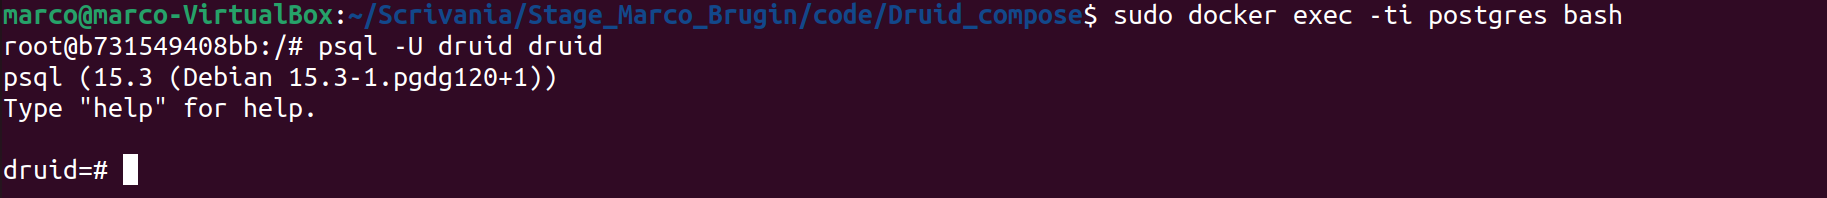
\includegraphics[width=1\textwidth]{images/percorso/accesso_psql.png}
  \caption{Connessione al database druid all'interno del container postgres}
  \label{fig:accesso_psql}
\end{figure}
\\
In seguito è stato anche eseguita l'\gls{injection}{} all'interno di \textbf{Apache Druid} 
andando a utilizzare l'interfaccia web, reperibile all'indirizzo
\textbf{http://localhost:8888/} (Figura \ref{fig:injection}).
\begin{figure}[h]
  \centering
  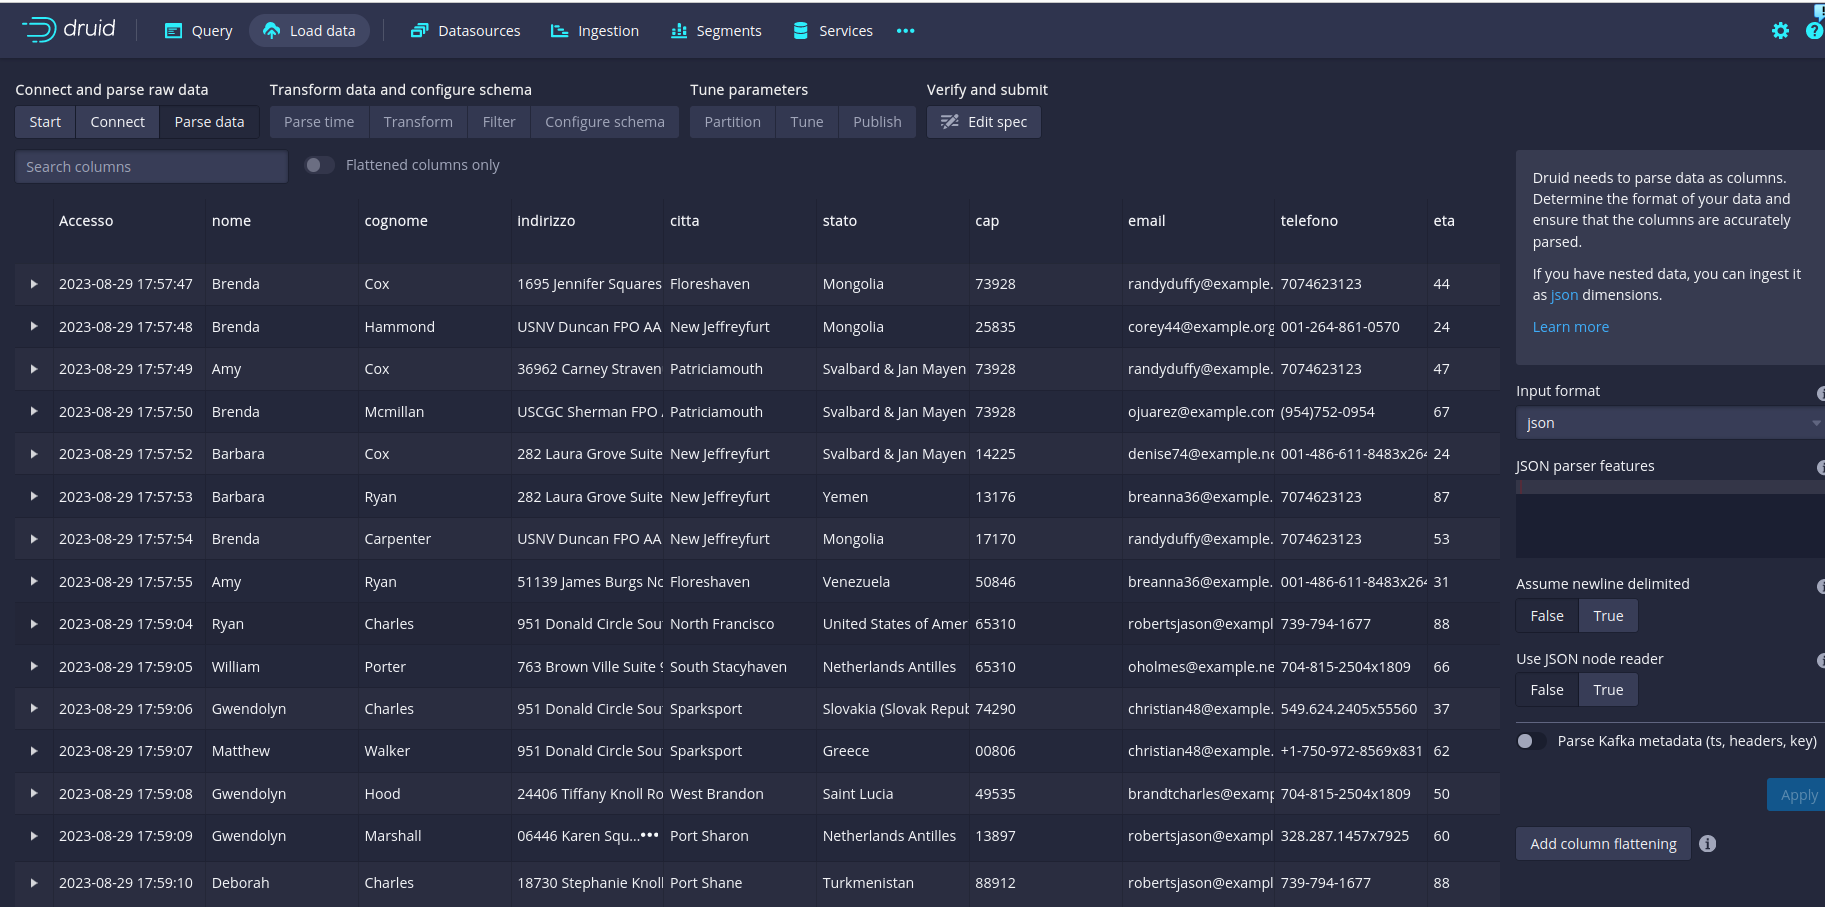
\includegraphics[width=1\textwidth]{images/percorso/load_data.png}
  \caption{Interfaccia web di Apache Druid per l'injection di un datasource}
  \label{fig:injection}
\end{figure}
\pagebreak
\\
In seguito sono state eseguite le seguenti query, sia su \textbf{Apache Druid} che su \textbf{PostgreSQL}.
\begin{lstlisting}[language=SQL, caption=\texttt{query.sql}, label=lst:file]{query.sql}
  - query 1: SELECT DATE_TRUNC('day', __time), citta, COUNT(*)
              FROM accessi
              GROUP BY DATE_TRUNC('day', __time), citta
       
 - query 2: SELECT stato, AVG(eta), AVG(reddito)
             FROM accessi
             GROUP BY stato
       
 - query 3: SELECT DATE_TRUNC('year', __time), stato, professione, istruzione, nfigli, COUNT(*)
             FROM accessi
             WHERE nfigli> 0
             GROUP BY DATE_TRUNC('year', __time), stato, professione, istruzione, nfigli
             ORDER BY 5 DESC
       
 - query 4: SELECT DATE_TRUNC('hour',__time), citta,  AVG(eta)
             FROM accessi
             GROUP BY DATE_TRUNC('hour', __time), citta  
 
 - query 5: SELECT DATE_TRUNC('year', __time), DATE_TRUNC('month', __time), DATE_TRUNC('day', __time), stato, professione, istruzione, nfigli, COUNT(*) 
         FROM accessi
         GROUP BY DATE_TRUNC('year', __time), DATE_TRUNC('month', __time), DATE_TRUNC('day', __time), stato, professione, istruzione, nfigli
         ORDER BY 5 DESC

 - query 6: SELECT DATE_TRUNC('year', __time), DATE_TRUNC('month', __time), DATE_TRUNC('day', __time), 
     DATE_TRUNC('hour', __time), stato, professione, istruzione, nfigli, COUNT(*) 
             FROM accessi
             GROUP BY DATE_TRUNC('year', __time), DATE_TRUNC('month', __time), DATE_TRUNC('day', __time), DATE_TRUNC('hour', __time), stato, professione, istruzione, nfigli
             ORDER BY 5 DESC           
 \end{lstlisting}
 \pagebreak
\subsubsection{Risultati}
I risultati ottenuti sono riportati nella tabella \ref{tab:risultati_query}.
\begin{table}[h]
  \centering
  \caption{Risultati delle query eseguite su Apache Druid e PostgreSQL}
  \label{tab:risultati_query}
  \begin{tabular}{|c|c|c|}


\hline
& \textbf{Apache Druid [s]} &  \textbf{PostgreSQL [s]} \\\hline 

\textbf{query1} &    0.6 &  1.2 \\ \hline

\textbf{query2} &   0.2 &   1.9 \\ \hline 

\textbf{query3} &  1.2 &  2 \\ \hline
\textbf{query4} &  0.6 &  1.1 \\ \hline
\textbf{query5} &   1.05 &  2.8 \\ \hline
\textbf{query6} & 1.30 &  3.3 \\ \hline    
  \end{tabular}
\end{table}
\subsubsection{Considerazioni}
Dai risultati ottenuti si può notare che \textbf{Apache Druid} ha prestazioni migliori rispetto a \textbf{PostgreSQL}.\\
Tale risultato è dovuto al fatto che \textbf{Druid} nella esecuzione delle query va a utilizzare solo le colonne richieste, grazie al fatto che 
il \gls{datasource}{} viene archiviato per singole colonne.\\
Inoltre si può notare anche che il divario delle prestazioni tra i due strumenti aumenta nel momento 
in cui si eseguono query che coinvolgono operazioni sui timestamp primari.
Infatti in \textbf{Druid} i dati vengono archiviati secondo un partizionamento temporale definito 
al momento dell'\gls{injection}{}, che permette di eseguire le query in modo efficiente (vedi \ref{sec:deep_storage}).
\pagebreak
\subsubsection{Confronto delle prestazioni di esecuzione tra datasource con e senza rollup in Apache Druid}\label{sec:confronto_prestazioni2}
Con il termine di \textbf{Data rollup} si intende un'operazione di aggregazione eseguita 
sui dati, che permette di ridurre la dimensione di questi ultimi, andando a creare dei record di archiviazione più piccoli e migliorando così 
le prestazioni di esecuzione delle query.\\
In \textbf{Apache Druid} l'operazione di \textbf{rollup}, viene eseguita attraverso la 
definizione di segmenti aggregati, creati in base a delle regole di aggregazione configurate al momento dell'\gls{injection}{} del \gls{datasource}{}, direttamente dall'interfaccia web di \textbf{Apache Druid} (Figura \ref{fig:rollup}).
\begin{figure}[h]
  \centering
  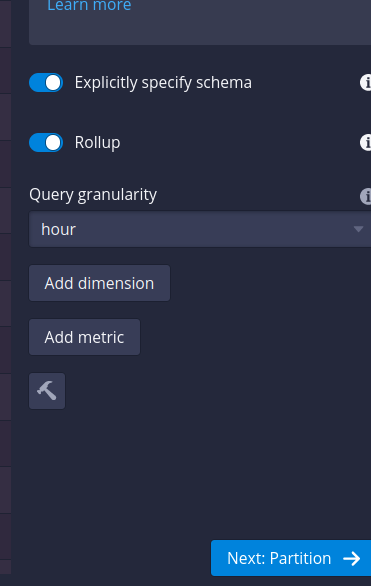
\includegraphics[width=0.3\textwidth]{images/percorso/test_rollup.png}
  \caption{Attivazione funzionalità di rollup all'interno di Apache Druid}
  \label{fig:rollup}
\end{figure}
\\
È importante sottolineare che l'operazione di \textbf{rollup} può essere configurata in base 
alla granularità temporale desiderata: si possono aggregare record aventi la stessa ora, minuti o secondi e considerando in seguito i  valori degli altri campi.\\
Per mettere in risalto la funzionalità appena descritta ho creato un \gls{datasource}{} di cinque milioni di record, come illustrato nel listato \ref{11st:file}.
\begin{lstlisting}[language=SQL,label=11st:file]
    CREATE TABLE accessi_rollup(__time timestamp, nome text, cognome text, citta text, stato text, datan date, istruzione text, hobby text)
\end{lstlisting}
In questo caso si tratta di un modello molto semplice 
e per riuscire ad apprezzare la funzionalità di \textbf{rollup} è stato ridotto
il numero di possibili valori, che ogni campo dati può assumere.\\
Pertanto il confronto è stato eseguito tra il \gls{datasource}{} originale e quello a cui è stata applicata la funzionalità di \textbf{rollup}.\\
Inoltre, per completezza, tutti i dati generati sono stati salvati e importati anche all'interno di \textbf{PostgreSQL} per avere 
anche un confronto con un classico \textbf{database relazionale}.

\pagebreak
\subsubsection{Svolgimento}
Per poter generare i dati necessari al \gls{datasource}{} sopra descritto, 
è stato utilizzato il produttore di eventi e la libreria \gls{Faker}{}, come illustrato nel listato \ref{l9st:file}.
\begin{lstlisting}[language=Python, caption=\texttt{producer\_rollup.py}, label=l9st:file]{producer.py}
  fake = Faker()
  locazione=[[fake.city(), fake.country()] for _ in range(200)]
  utenti=list()
  num_utenti=5000
  for i in range(num_utenti):
      loc=locazione[random.randint(0,199)]
      citta=loc[0]
      stato=loc[1]
      utenti.append([fake.first_name(), fake.last_name(),fake.date_of_birth(minimum_age=18, maximum_age=89).strftime("%Y-%m-%d"), citta, stato, fake.random_element(elements=("Scuola Secondaria", "Laurea triennale", "Laurea Magistrale", "Dottorato")), fake.random_element(elements=("Leggere","Viaggiare","Giocare a calcio","Giocare ai videogiochi","Fare sport")) ] )
  for n in range(50):
    for j in range(100000):
        accesso=datetime.datetime.now().strftime("%Y-%m-%d %H:%M:%S")
        a=random.randint(0,4999)
        nome=utenti[a][0]
        cognome=utenti[a][1]
        datan=utenti[a][2]
        citta=utenti[a][3]
        stato=utenti[a][4]
        istruzione=utenti[a][5]
        hobby=utenti[a][6]
        my_data = {"__time": accesso, "nome": nome, "cognome": cognome, "datan":  datan, "citta": citta, "stato": stato, "istruzione": istruzione,
        "hobby": hobby
        }
        producer.send("rollup", value = my_data) 
    \end{lstlisting}
In seguito sono state eseguente le seguenti query su i tre \gls{datasource}{} creati.
\begin{lstlisting}[language=SQL, caption=\texttt{query\_rollup.sql}, label=lst:file]{query_rollup.sql}
  - query 1: SELECT DATE_TRUNC('day', __time), citta, COUNT(*)
              FROM accessi_rollup
              GROUP BY DATE_TRUNC('day', __time), citta
              
  - query 2: SELECT DATE_TRUNC('year', __time), DATE_TRUNC('month', __time), stato, COUNT(*)
              FROM accessi_rollup
              GROUP BY DATE_TRUNC('year', __time), DATE_TRUNC('month', __time), stato
              ORDER BY 4 DESC
  
  - query 3: SELECT DATE_TRUNC('year', __time), DATE_TRUNC('month', __time), DATE_TRUNC('day', __time), stato, citta, COUNT(*) 
              FROM accessi_rollup
              GROUP BY DATE_TRUNC('year', __time), DATE_TRUNC('month', __time), DATE_TRUNC('day', __time), stato, citta
              ORDER BY 5 DESC
  
  - query 4: SELECT DATE_TRUNC('year', __time), DATE_TRUNC('month', __time), DATE_TRUNC('day', __time), DATE_TRUNC('hour', __time), stato, citta, COUNT(*) 
              FROM accessi_rollup
              GROUP BY DATE_TRUNC('year', __time), DATE_TRUNC('month', __time), DATE_TRUNC('day', __time), DATE_TRUNC('hour', __time), stato, citta
              ORDER BY 5 DESC
  \end{lstlisting}
\subsubsection{Risultati}
I risultati ottenuti sono riportati nella tabella \ref{tab:risultati_rollup}.
\begin{table}[h]
  \centering
  \caption{Risultati delle query eseguite con, senza rollup e su PostgreSQL}
  \label{tab:risultati_rollup}
  \begin{tabular}{|c|c|c|c|}
  \hline
 & \textbf{Apache Druid}  & \textbf{Apache Druid} & \textbf{PostgreSQL}  \\
& \textbf{ con rollup [s]} & \textbf{ senza rollup [s]}  & \textbf{ [s]} \\\hline
  \textbf{query1} &   0.3  &  0.7 &  0.8 \\ \hline
  \textbf{query2} &  0.4 &  0.75 &  1.1 \\ \hline
  \textbf{query3} &   0.25   &  0.74  &  1.5 \\ \hline
  \textbf{query4} &   0.16   &  0.8  &  1.6 \\ \hline
  \end{tabular}
\end{table}
\subsubsection{Considerazioni}
Dai risultati ottenuti si può notare che l'operazione di \textbf{rollup} 
permette di migliorare in modo considerevole le prestazioni di esecuzione delle query, all'interno di \textbf{Apache Druid}.\\
Infatti se si confrontano le cardinalità dei due \gls{datasource}{} con e senza \textbf{rollup} si nota che da cinque milioni di record iniziali
si arriva a centocinquantamila record aggregati, permettendo così una riduzione considerevole del volume di dati da analizzare.\\
Infine si sottolinea che la funzionalità di \textbf{rollup} non fa altro che aumentare il divario tra \textbf{Apache Druid} e un 
classico database relazionale, come \textbf{PostgreSQL}.
\pagebreak
\subsection{Utilizzo delle tabelle di lookup in Apache Druid}
Con il termine di tabelle di \textbf{lookup} si intende un funzionalità che consente di sostituire i valori 
di un determinato attributo di un \gls{datasource}{} con un altro valore, definito all'interno di una tabella di \textbf{lookup}.\\
Più in generale tale processo prende il nome di \textbf{Data enrichment}: processo di miglioramento, ampliamento o arricchimento dei dati esistenti con informazioni 
aggiuntive provenienti da diverse fonti. \\
In \textbf{Apache Druid} le tabelle di \textbf{lookup} sono costituite da un campo \textbf{chiave} a cui viene associato un campo \textbf{valore} che andrà a sostituire la chiave.\\
Inoltre è necessario sottolineare che le tabelle di \textbf{lookup} non hanno cronologia e lavorano indipendentemente dall'intervallo di tempo su cui si esegue la query: restituiscono sempre il dato corrente.\\
Per poter sperimentare tale funzionalità ho creato un \gls{datasource}{} di cinquecento record, come delineato nel listato \ref{l4st:file}.
\begin{lstlisting}[language=SQL,label=l4st:file]
  CREATE TABLE accessi_lookup(__time timestamp, citta text, stato text, codice_cliente text);
\end{lstlisting}
In questo caso la tabella di \textbf{lookup} è stata utilizzata per  sostituire al \textit{codice\_cliente}, il \textit{nome} e il \textit{cognome} del cliente stesso.
\subsubsection{Svolgimento}
Per poter generare i dati necessari al \gls{datasource}{} sopra descritto, è stato utilizzato un produttore di eventi 
analogo a quelli descritti nelle sezioni \ref{sec:confronto_prestazioni1} e \ref{sec:confronto_prestazioni2}.\\
In questo caso è importante sottolineare che, dopo aver generato i dati necessari, tutti i 
record  creati sono stati salvati per effettuare la creazione della tabella di \textbf{lookup} (Figura \ref{fig:lookup}).\\
\begin{figure}[h]
  \centering
  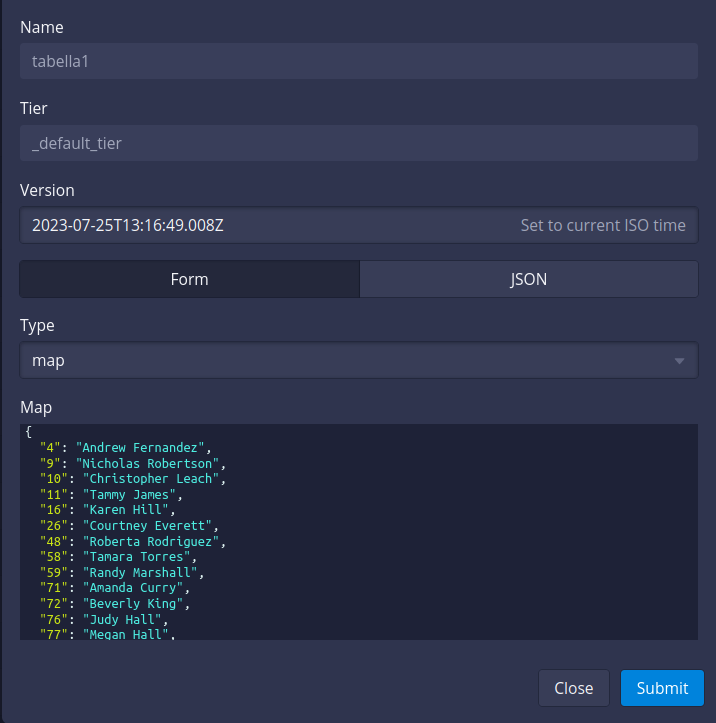
\includegraphics[width=0.6\textwidth]{images/percorso/inserimento_lookup.png}
  \caption{Creazione della tabella di lookup all'interno di Apache Druid}
  \label{fig:lookup}
\end{figure}
\pagebreak
\\
In seguito per poter testare tale funzionalità è stata eseguita la seguente query.
\begin{lstlisting}
  SELECT LOOKUP(codice_cliente,'tabella1'), datan, citta, stato
  FROM accessi_lookup
\end{lstlisting}
Si sottolinea che, per poter utilizzare le tabelle di \textbf{lookup} in \textbf{Apache Druid}, 
è necessario
inserire all'interno della query desiderata la funzione \textbf{LOOKUP}, riportando come primo parametro il campo chiave della tabella di \textbf{lookup} e come secondo parametro il nome della tabella stessa.\\
\subsubsection{Risultati}
Il risultato ottenuto è illustrato in Figura \ref{fig:risultato_lookup}.
\begin{figure}[h]
  \centering
  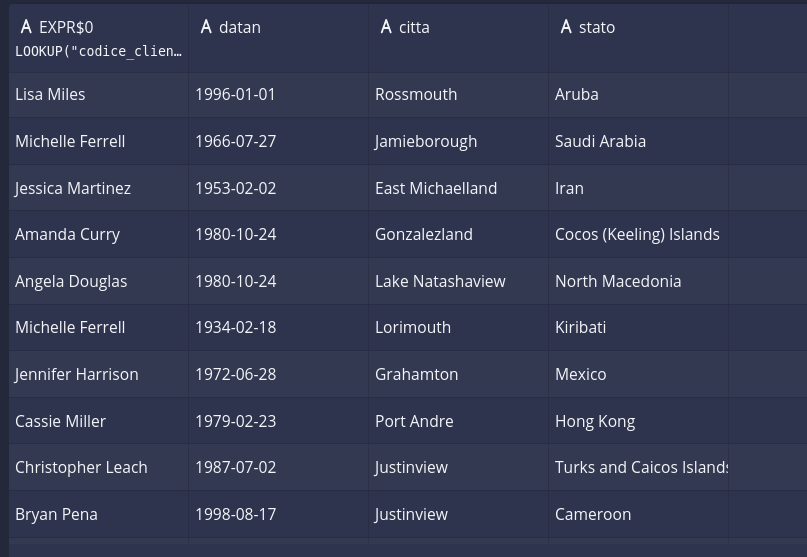
\includegraphics[width=1\textwidth]{images/percorso/lookup.png}
  \caption{Risultato della query eseguita con la funzionalità di lookup}
  \label{fig:risultato_lookup}
\end{figure}
\subsubsection{Considerazioni}
Dai risultati ottenuti 
si sottolinea che per ottenere lo stesso risultato all'interno di un classico \textbf{database relazionale}
è necessario ricorrere all'unione tra due tabelle, operazione che risulta essere molto onerosa.
\pagestyle{empty}
\null % o \mbox{} o \phantom{X}
\newpage
    \chapter{Valutazioni e Conclusioni}
\label{cap:conclusioni}

\section{Consuntivo finale}

\section{Raggiungimento degli obiettivi}

\section{Conoscenze acquisite}

\section{Valutazione personale}


    \appendix

    \backmatter
    \printglossary[type=\acronymtype, title=Acronimi e abbreviazioni, toctitle=Acronimi e abbreviazioni]
    \printglossary[type=main, title=Glossario, toctitle=Glossario]

    \cleardoublepage
\chapter{Bibliografia}

\nocite{*}

% Print book bibliography
\printbibliography[heading=subbibliography,title={Riferimenti bibliografici},type=book]

% Print site bibliography
\printbibliography[heading=subbibliography,title={Siti web consultati},type=online]

\end{document}
